\documentclass[journal, twoside]{IEEEtran}
\let\labelindent\relax

% math related package
\usepackage{amsmath}
\usepackage{amssymb}
\usepackage{mathtools}
\usepackage{eqlist}
\usepackage{amsfonts}
%% math -- mathbold
\def\mathbi#1{\textbf{\em #1}}
%% math -- observation command
\usepackage{amsthm}
\newtheorem*{observation}{Important Observation}
% table related package
\usepackage{tabularx}
\usepackage{threeparttable}
\usepackage{booktabs}
\usepackage{makecell}
\usepackage{colortbl}
% figure related package
\usepackage{graphicx}
\usepackage{wrapfig}
\usepackage{subcaption}
% algorithm related package
\usepackage[lined, ruled, linesnumbered, commentsnumbered, noend]{algorithm2e}
\usepackage[colorlinks=true, allcolors=blue]{hyperref}
\newcommand\mycommfont[1]{\footnotesize\ttfamily\textcolor{blue}{#1}}
\renewcommand{\thefootnote}{\tiny~Note \arabic{footnote}}
\SetCommentSty{mycommfont}
% formatting related package
\usepackage{enumitem}
\usepackage{lipsum}
\usepackage{stfloats}
\usepackage{ulem}
\normalem
\usepackage[numbers]{natbib}
\usepackage[usenames,dvipsnames]{xcolor}
\usepackage{comment}
\usepackage{flushend}
%% formatting -- multirow underline
\usepackage{multirow}
\newcommand\dunderline[3][-2pt]{{%
  \setbox0=\hbox{#3}
  \ooalign{\copy0\cr\rule[\dimexpr#1-#2\relax]{\wd0}{#2}}}}
% how to broke words
\hyphenation{}
% displacement
\usepackage{tikz}
\usetikzlibrary{fit, shapes.misc}
\newcommand\marktopleft[1]{%
    \tikz[overlay,remember picture]
        \node (marker-#1-a) at (0,1.5ex) {};%
}
\newcommand\markbottomright[1]{%
    \tikz[overlay,remember picture]
        \node (marker-#1-b) at (0,0) {};%
    \tikz[overlay,remember picture,thick,inner sep=3pt]
        \node[draw, rectangle, color=teal, fit=(marker-#1-a.center) (marker-#1-b.center)] {};%
}
\newcommand{\circnum}[1]{\raisebox{0.2ex}{\textcircled{\raisebox{-0.2ex}{#1}}}}
% colored box
\newcommand{\limebox}[1]{\setlength{\fboxsep}{0pt}{\colorbox{lime}{#1}}}
\newcommand{\pinkbox}[1]{\setlength{\fboxsep}{0pt}{\colorbox{yellow}{#1}}}
% international fonts
\usepackage{CJKutf8}
% check and revision
\definecolor{bleudefrance}{rgb}{0.19, 0.55, 0.91}
\definecolor{awesome}{rgb}{1.0, 0.13, 0.32}
\definecolor{darkgreen}{rgb}{0.0, 0.65, 0.0}
\definecolor{babyblue}{rgb}{0.29, 0.75, 0.93}
\newcommand{\wan}[1]{{\color{purple}\begin{CJK*}{UTF8}{gkai}#1\end{CJK*}}}
\newcommand{\wanex}[1]{{\color{violet}\begin{CJK*}{UTF8}{gkai}#1\end{CJK*}}}
\newcommand{\wanexex}[1]{{\color{brown}\begin{CJK*}{UTF8}{gkai}#1\end{CJK*}}}
\newcommand{\wanfinal}[1]{{\color{blue}\begin{CJK*}{UTF8}{gkai}#1\end{CJK*}}}
\definecolor{darkorange}{rgb}{1.0, 0.55, 0.0}
\newcommand{\xinyi}[1]{{\color{darkorange}\begin{CJK*}{UTF8}{gkai}#1\end{CJK*}}}
\newcommand{\xinyitodo}[1]{{\color{darkgreen}\begin{CJK*}{UTF8}{gkai}#1\end{CJK*}}}
\newcommand{\harada}[1]{\textcolor{green}{#1}}
\newcommand{\recheck}[1]{\textcolor{olive}{#1}}
\newcommand{\rev}[1]{\begingroup\color{magenta}#1\endgroup}
% (\rev) uppercase alias: IEEEtran \MakeUppercase's the running head, which
% would otherwise turn \color{magenta} into the undefined \color{MAGENTA}.
\definecolor{MAGENTA}{cmyk}{0,1,0,0}

\begin{document}
\title{Extreme Motion Generation \\via Learning-Based Null-Space Control\\ for Straight-Line Path Following}
\author{Xinyi Yuan, Weiwei Wan$^{*}$, Kensuke Harada
\thanks{Department of System Innovation, Graduate School of Engineering Science, The University of Osaka, Toyonaka, Osaka, Japan.}
\thanks{$^{*}$Contact: Weiwei Wan, {\tt\small wan@sys.es.osaka-u.ac.jp}}}
\markboth{IEEE Transactions on Automation Science and Engineering, 2026.}
{Yuan \MakeLowercase{\textit{et al.}}: Extreme Motion Generation via Learning-Based Null-Space Control for Straight-Line Path Following}
\maketitle

\bstctlcite{IEEEexample:BSTcontrol}
%%%%%%%%%%%%%%%%%%%%%%%%%%%%%%%%%%%%%%%%%%%%%%%%%%%%%%%%%%%%%%%%%%%%%%%%%%%%%%%%
\begin{abstract}
This work studies \textit{extreme motion generation}, which aims to maximize the Cartesian path length along a pre-defined trajectory within the manipulator's workspace. This objective is important in industry as path-following is fundamental to a large variety of tasks such as surface coating and welding. More critically, extreme motion enables a fixed-base manipulator to exploit the kinematic capability under limited reachability. However, such exploitation is challenging in practice, as the manipulator must actively avoid the safety boundary through execution, which is inherently a long-horizon problem. \xinyi{Accordingly, we claim that a learning-based policy capable of long-horizon decision-making should maximize exploitation within the interior safe region while carefully avoiding joint-limit violations near the boundary. In detail, we first construct an expert hybrid policy whose model-based controller takes over near the joint limits, where the learning-based policy fails under sparse data coverage. We then distill this expert into a single learning-based policy, which in turn constitutes a stronger expert in the next iteration, thereby closing the expert-iteration loop.} The initial joint configuration \xinyi{selection} is \xinyi{based on} the conditional diffusion-based sampling, which improves the achievable path length based on the learned motion prior. We evaluate the proposed framework on 10,000 straight-line path-following tasks with a 7-DoF Franka FR3, \xinyi{recovering 98.2\% of the per-task reference length and extending the average path length by 39\% over the model-based baseline.} The project website and related videos of this paper can be found at \url{https://yuan-xinyi.github.io/extreme-motion-generation/}.

% Notably, certain tasks yield a pronounced extension toward the motion extreme, as reflected in the maximum improvement reported in the statistical results.

\end{abstract}

\begin{IEEEkeywords}
extreme motion generation, reinforcement learning\xinyi{, policy distillation.}
\end{IEEEkeywords}

\section{Introduction}
Consider a compact, fixed-base manipulator executing a coating or welding operation over a large work surface. Given a starting position and a motion direction, intuition would suggest that the maximum reachable point is determined by the reachable workspace. However, the motion is continuous and strictly constrained by safety boundaries such as joint limits and tool-orientation tolerance along each waypoint. Therefore, the practical bottleneck is that one of those safety constraints is violated and causes termination long before the end-effector approaches the edge of the reachable workspace. Consequently, the practically achievable path length is influenced by how long the safety boundaries can be deferred from being met during the motion execution process. We refer to this problem as \textit{extreme motion generation} that maximizes the Cartesian path length along a pre-defined trajectory within the manipulator's workspace. This is particularly important in industrial automation, where the length of a single continuous motion directly limits the area a manipulator can process in one setup. Rather than scaling up the manipulator or repeatedly relocating the base, simply exploiting the extreme motion offers a solution to enlarge the effective working range.

However, extreme motion generation, especially under precise path-following, is challenging in practice. The joint motion at the current step may gradually steer the subsequent motion toward a safety boundary, ultimately forcing it to terminate. Therefore, the problem is inherently a long-term decision-making problem, as each step must account for its consequences over the entire motion. Unfortunately, current motion generation tools have certain drawbacks with respect to the requirement of both robustness and exploitation. On the one hand, a classical controller optimizes an instantaneous secondary objective while realizing the desired end-effector motion. Such controllers are myopic, optimizing an instantaneous surrogate and overlooking its long-horizon consequences. Yet near the joint limits, their behavior is robust and predictable by design. On the other hand, the learning-based policy is designed to have the foresight suitable for exploitation. However, the learning paradigm is based on probabilistic distribution approximation, and near-boundary configurations are rarely sampled. As a result, the derived policy is particularly fragile near the boundary regions that are most critical to extreme motion generation.

Motivated by this complementarity, we delegate the long-horizon decision-making in the well-sampled interior to a Reinforcement-Learning (RL) policy, where foresight can be trusted. The near-boundary region is handled by the classical controller, whose robustness is guaranteed by construction. The two regimes are coordinated at every control step by a hysteresis rule on the normalized joint-limit distance, ensuring that each model operates within the region where it is most reliable. In addition, a conditional diffusion model initializes the manipulator on a robust starting configuration prior to execution of the hybrid controller.

\rev{Building on this complementarity, we further improve the learning-based controller through expert iteration: the hybrid controller serves as an expert that is distilled into a single policy of the same architecture as the RL policy, and the improved policy in turn constitutes a stronger expert, so that the learned controller progressively internalizes the near-boundary behavior that reinforcement learning alone can neither discover nor retain. For the initialization, we observe that the diffusion samples generated for a task land on different branches of the self-motion manifold whose reachable path lengths differ sharply, so that selecting among the samples is as important as generating them. We therefore equip the diffusion prior with a learned scorer that selects the most promising candidate before execution, under a strict deployment budget of no additional rollouts and a single selection per task.}

We evaluate the proposed framework on a large set of straight-line path-following tasks for a 7-DoF Franka FR3, measuring performance as the achieved path length relative to a per-task reference length. The contribution of each component is then analyzed through the seed-by-controller protocol. For the initial joint configuration, the diffusion-based selection is compared against several hand-designed heuristic seeds; for the controller, the hybrid framework is compared against the classical and the learning-based controllers in isolation. We further conduct ablation studies on the guidance scale, the number of diffusion sampling steps, \rev{the hysteresis switching thresholds, and the convergence of the expert iteration}, providing practical insights into the effect of each design choice.

\section{Related Work}

\subsection{Manipulability and Reachability}
Extreme motion generation is essentially related to the manipulator's reachable workspace and local motion dexterity during motion execution. Manipulability and reachability describe local instantaneous motion dexterity and global spatial feasibility, respectively.

The manipulability ellipsoid \cite{yoshikawa1985manipulability} characterizes the relationship between joint and task-space velocities via the Jacobian, and its projection along a task direction quantifies directional capability. To exploit this measure online, Jin et al.~\cite{jin2017manipulability} adopted a dynamic neural network for inverse-free manipulability optimization. Recent work integrates manipulability into planning: Shen et al.~\cite{shen2023adaptive} proposed a manipulability-aware $\text{RRT}^{\star}$ that embeds the measure into both cost and step size, and Cai et al.~\cite{cai2025just} balanced path cost against manipulability to mitigate singularities during planning. The above studies can effectively keep the manipulator away from singular configurations but act only on the instantaneous state and overlook the long-horizon consequences of the current motion.

Complementary to local dexterity, reachability analysis delineates the global spatial limit that bounds how far any motion can extend. Early studies established geometric \cite{yang2009placement} and voxel-based \cite{makhal2018reuleaux} reachability maps to automate base placement without exhaustive IK. Moving toward dynamic settings, Feng et al.~\cite{feng2025predictive} introduced predictive reachability via world models for embodiment selection, while Jauhri et al.~\cite{jauhri2022robot} used reachability priors to accelerate RL-based control, and Selim et al.~\cite{selim2022safe} proposed a reachability-based safety layer with formal guarantees. These methods characterized the reachable space with a static, precomputed envelope. However, they do not address how to actively defer the safety boundaries during execution so that the end-effector approaches this envelope as closely as possible. Bridging this gap is precisely the goal of extreme motion generation.

\subsection{Learning-based Motion Generation}
In contrast to optimizing an instantaneous objective, learning-based methods capture the multi-modal distribution of feasible configurations and enable long-horizon motion generation. For example, Reinforcement Learning (RL) has been applied to redundancy resolution \cite{malik2022deep}, and generative solvers such as IKFlow \cite{ames2022ikflow} and IKDiffuser \cite{zhang2025ikdiffuser} modeled the full solution manifold rather than a single solution. The related study DiffusionSeeder \cite{huang2024diffusionseeder} utilized generative models to seed downstream motion to produce multi-modal trajectory initializations, and Yoon et al.~\cite{yoon2023learning} proposed an RL-based initialization generator.

\xinyitodo{需要补充更多基于学习的learning的论文，尤其是path following}

Such learned priors supply the foresight that manipulability- and reachability-based methods lack. However, the data used to train these policies is sparsely distributed near the kinematic boundaries. Consequently, the resulting policies are most fragile in exactly the near-boundary region that is most critical to extreme motion generation. This complementarity between learned foresight in the well-sampled region and classical robustness near the boundary motivates the proposed hybrid framework.

\subsection{Combining Learning- and Model-based Control}
To address the aforementioned issues, the solution could be to combine a learned policy with a model-based controller. One line of work combines the output actions additively: residual RL keeps a fixed classical controller and learns a corrective action added on top of that \cite{johannink2019residual,silver2018residual}. Another line of research switches between different controllers by safety criteria or pre-defined regions. For example, Mehmood et al.~\cite{mehmood2022black} switched to a verified backup controller under runtime reachability checks. Similarly, Alshiekh et al.~\cite{alshiekh2018safe} proposed to override unsafe learned actions whenever the agent approaches the boundary. Likewise, Kurtz et al.~\cite{kurtz2021control} continuously filtered the nominal action to keep it within a safe set, as in control-barrier-function safety filters for manipulators.

Generally, our framework follows the switching rather than the additive paradigm. Similar to the safety-driven methods above, we trigger the backup classical controller near the safety boundary. However, our motivation is not merely to stay safe but to keep advancing the motion toward its kinematic limit, which is the core objective of extreme motion generation. Accordingly, we partition the configuration space by proximity to the joint-limit boundary and assign each region to the controller most reliable there.


\subsection{\xinyi{Learning-Based Policy Improvement}}
\rev{When a learned policy is imperfect, a range of methods improve it beyond what its original training objective attains. Imitation-based methods correct a policy from a reference behavior: DAgger~\cite{ross2011reduction} addresses the distribution shift of behavior cloning by repeatedly querying the reference on the states the current policy actually visits and aggregating them into the training set, so that the policy is corrected exactly where it drifts. When a stronger reference is available in the form of an expert whose performance is known to be superior, policy distillation~\cite{rusu2015policy} compresses that expert into the deployed network, letting the network approximate the expert as closely as its capacity allows. Expert iteration~\cite{anthony2017thinking} combines the two ideas into a loop: an expert is constructed around the current policy, the policy is distilled from that expert, and the improved policy in turn constitutes a stronger expert for the next round, so that the policy and its expert improve together until the expert no longer surpasses the policy. Guided policy search~\cite{levine2013guided} follows a related principle, distilling a trajectory-optimization expert into a reactive policy. Our framework instantiates expert iteration with the hybrid controller as the expert, as detailed below.}




% \section{Preliminaries}
\section{Problem Formulation}
While extreme motion generation applies broadly to constrained path following, we here specify it as extreme straight-line path following. Specifically, a fixed-base manipulator advances its end-effector along the line with a tool-orientation constraint. As illustrated in Fig.~\ref{overview}, solving this problem requires first determining the initial joint configuration from which the motion starts and then generating the motion that maximizes the achievable path length.

\begin{figure*}[!htbp]
    \centering
    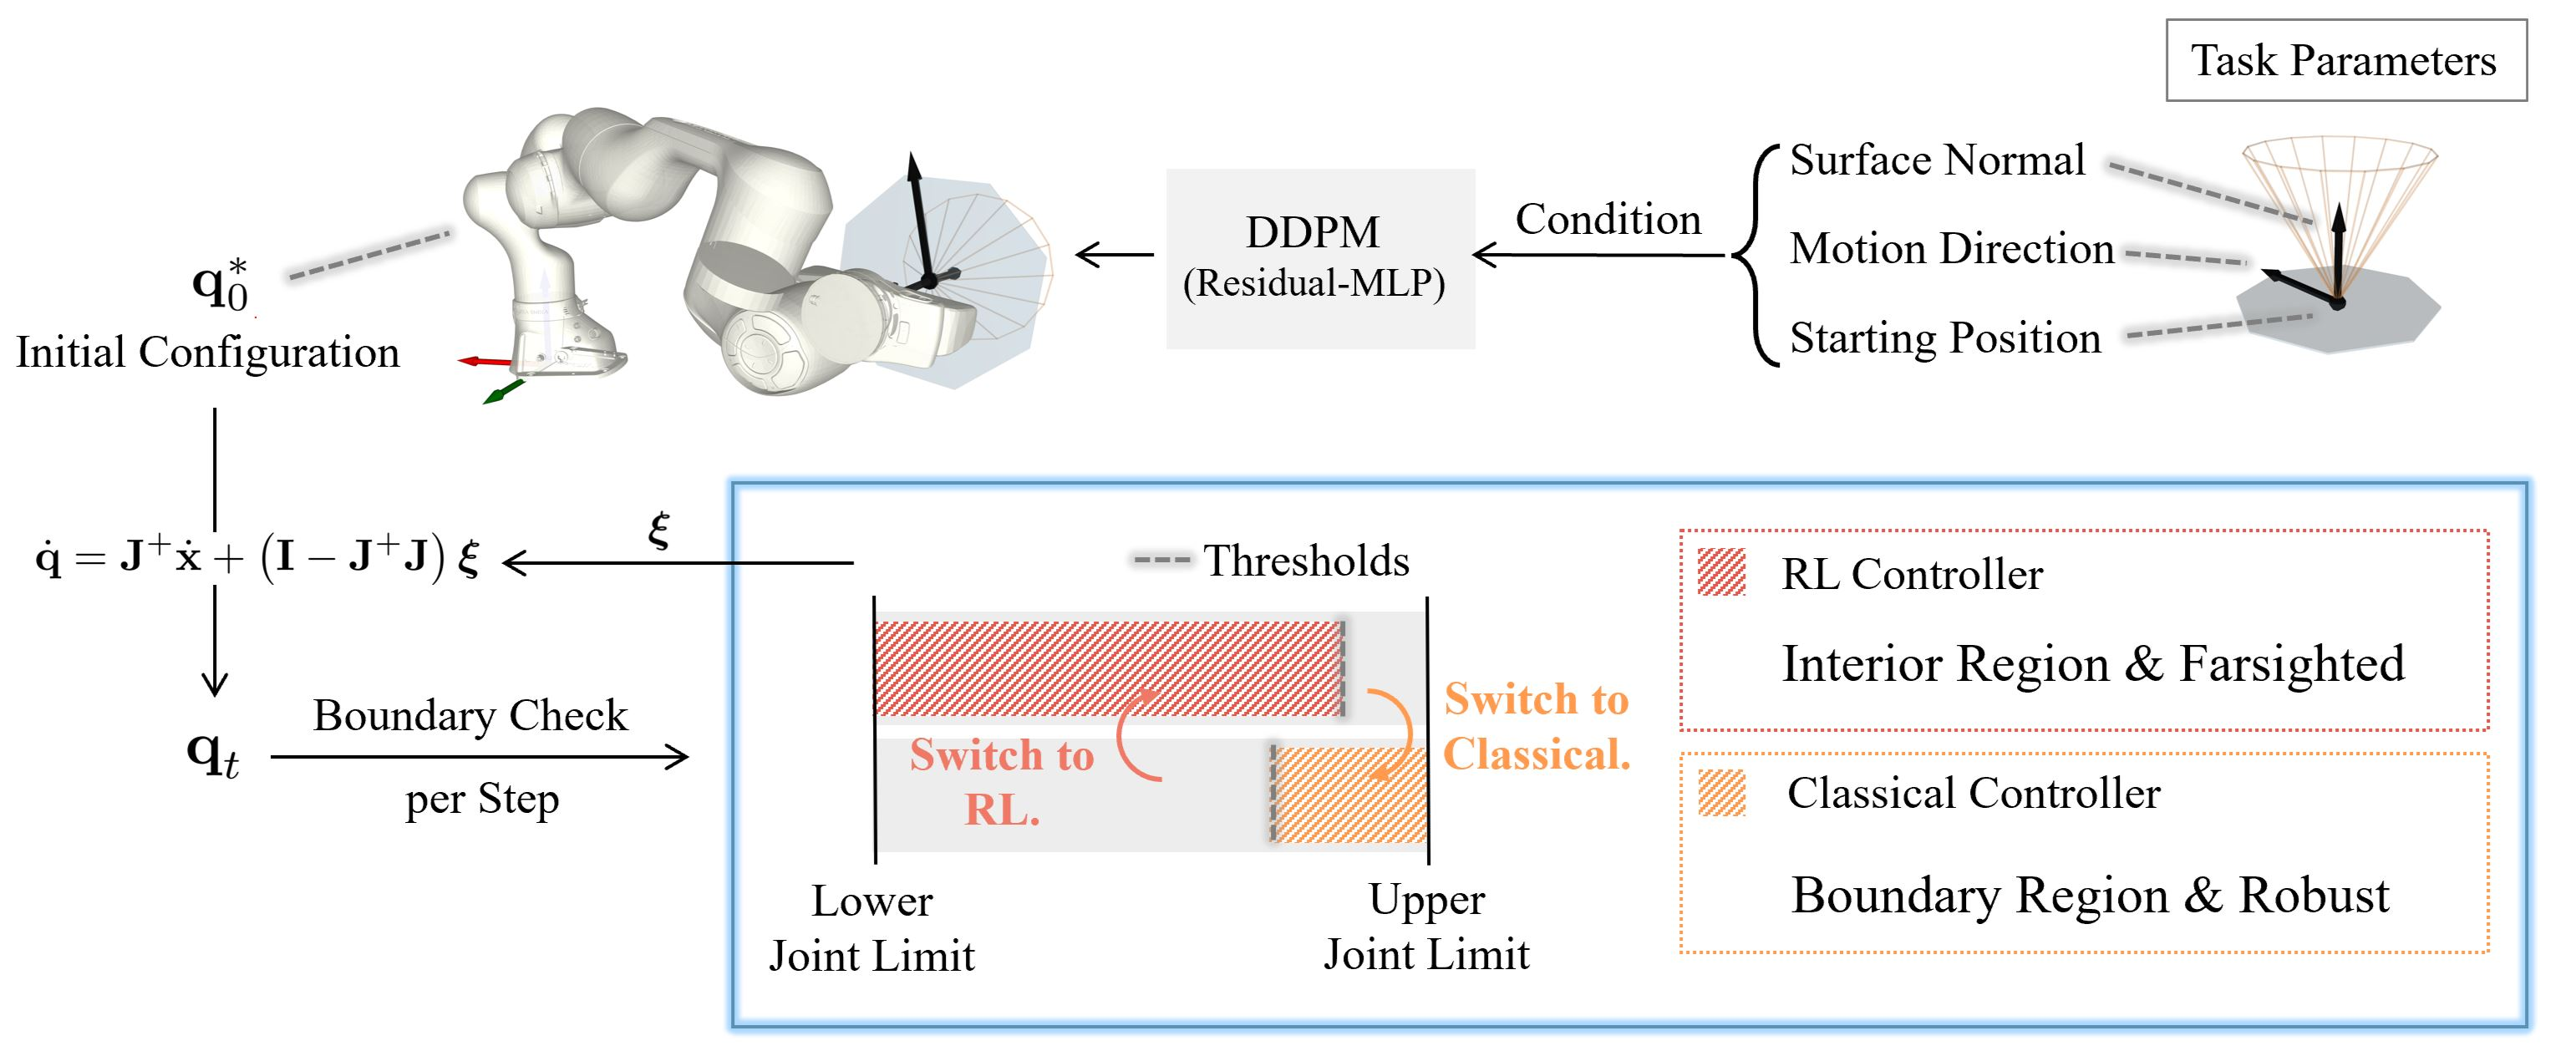
\includegraphics[width=\linewidth]{imgs/system_overview.JPG}
    \caption{Overview of the two-stage framework for extreme motion generation.}
    \label{overview}
\end{figure*}

We formalize the above task as follows. Consider a manipulator with $n$ degrees of freedom, where $\mathbf{q} \in \mathbb{R}^{n}$ denotes the joint configuration. Let $\mathbf{p}(\mathbf{q}) \in \mathbb{R}^{3}$ denote the end-effector position and $\mathbf{z}(\mathbf{q}) \in \mathbb{R}^{3}$ denote the TCP local $z$-axis. A straight-line path-following task is specified by the condition vector:
\begin{equation}
\label{cond}
\mathbf{c} = [\mathbf{p}_{0}, \mathbf{d}, \mathbf{n}] \in \mathbb{R}^{9},
\end{equation}
where $\mathbf{p}_{0}$ denotes the starting position, and $\mathbf{d}$ and $\mathbf{n}$ are unit vectors representing the desired motion direction and task-plane normal, respectively. 

Starting from an initial configuration $\mathbf{q}_{0}^{*}$, the policy $\pi$ determines the joint motion at every control step to maximize the path-following length, producing a joint trajectory $\{\mathbf{q}_{t}^{*}\}_{t=0}^{T}$ initialized at $\mathbf{q}_{0}^{*}$, where $T$ is the termination step at which any safety constraint is first violated. This task can be formalized as a constrained optimization problem as:
\begin{align}
\max_{\mathbf{q}_{0}^{*},\,\pi} \quad & \mathcal{L}(\mathbf{q}^{*}_{0},\,\pi;\,\mathbf{p}_{0}, \mathbf{d}, \mathbf{n}) \\
\text{s.t.} \quad & \|\mathbf{p}(\mathbf{q}_{t}^{*}) - \mathbf{p}_{t}\| \leq \epsilon_{\text{pos}}, \\
& \arccos\!\left( \mathbf{z}(\mathbf{q}_{t}^{*})^{\top} \mathbf{n} \right) \leq \theta_{\max}, \label{eq:ori_constraint} \\
& \mathbf{q}_{\min} \preceq \mathbf{q}_{t}^{*} \preceq \mathbf{q}_{\max}, \label{eq:jl_constraint}
\end{align}
where $\mathcal{L}$ denotes the path-following length, $\mathbf{q}_0^*$ and $\pi$ are the initial configuration and the control policy to be optimized, and $(\mathbf{p}_0, \mathbf{d}, \mathbf{n})$ specify the task conditions as above. The $\epsilon_{\text{pos}}$, $\theta_{\max}$, and $[\mathbf{q}_{\min}, \mathbf{q}_{\max}]$ are the position tolerance, orientation tolerance, and joint limits, respectively.

During this process, since only the $3$-DoF end-effector position must be precisely tracked, the remaining freedom makes the manipulator kinematically redundant for $n>3$. This redundancy is resolved in the null space of the position Jacobian, which decomposes the commanded joint velocity into a task term and a null-space term,
\begin{equation}
\label{eq:nullspace}
\dot{\mathbf{q}} = \mathbf{J}^{+}\dot{\mathbf{x}} + (\mathbf{I}-\mathbf{J}^{+}\mathbf{J})\,\boldsymbol{\xi},
\end{equation}
where $\mathbf{J}^{+}$ is the damped pseudo-inverse and $(\mathbf{I}-\mathbf{J}^{+}\mathbf{J})$ projects the secondary command $\boldsymbol{\xi}$ onto the null space. Within this null space, several secondary objectives can be pursued without disturbing the end-effector position:
\begin{equation}
\label{eq:secondary}
\boldsymbol{\xi}=k_{\mu}\,\nabla_{\mathbf{q}}w_{\mathbf{d}}(\mathbf{q})\;-\;k_{\mathrm{jl}}\,\frac{\mathbf{q}-\mathbf{q}_{\mathrm{mid}}}{\mathbf{q}_{\max}-\mathbf{q}_{\min}}\;+\;k_{\theta}\,g(\theta)\,\nabla_{\mathbf{q}}\!\big(\mathbf{z}(\mathbf{q})^{\top}\mathbf{n}\big),
\end{equation}
where the secondary command $\boldsymbol{\xi}$ combines a directional-manipulability term $w_{\mathbf{d}}$ that retreats from singularities along $\mathbf{d}$, a centering term that pulls each joint toward the middle $\mathbf{q}_{\mathrm{mid}}$ of its range, and a cone term gated by $g(\theta)$ that activates only as the tool axis approaches the $\theta_{\max}$ boundary. Notably, all subsequent controllers share this task decomposition, differing only in the strategy used to generate the secondary command $\boldsymbol{\xi}$.

% \subsection{Task Optimization via Null-Space Control}
% \wan{零空间控制属于常识，有必要做前提知识吗？}\xinyi{可删除章节。}\wan{把下一节开头的任务具化放在这里，具化完后简单讲一下零空间。}
% \label{sec:baseline}
% % here to state how is the joint velocity be decomposed, and how is the null space been improved via gradient asent. List the fomulars. the detailed formulas can be put in the appendix
% For a manipulator, the position Jacobian $\mathbf{J}(\mathbf{q})=\partial\mathbf{p}/\partial\mathbf{q}\in\mathbb{R}^{3\times n}$ has a non-trivial null space, so the joint velocity that realizes a desired end-effector motion is not unique. The classical controller decomposes the commanded joint velocity into a task term and a null-space term,
% \begin{equation}
% \label{eq:nullspace}
% \dot{\mathbf{q}} = \mathbf{J}^{+}\dot{\mathbf{x}} + \big(\mathbf{I}-\mathbf{J}^{+}\mathbf{J}\big)\,\boldsymbol{\xi},
% \end{equation}
% where $\mathbf{J}^{+}=\mathbf{J}^{\top}(\mathbf{J}\mathbf{J}^{\top}+\lambda^{2}\mathbf{I})^{-1}$ is the damped pseudo-inverse with a Nakamura--Hanafusa adaptive damping $\lambda$ that grows only as the smallest singular value of $\mathbf{J}$ drops below a threshold, and $\mathbf{I}-\mathbf{J}^{+}\mathbf{J}$ projects the secondary command $\boldsymbol{\xi}$ onto the null space. 

% For the straight-line path following task in this study, the task velocity $\dot{\mathbf{x}}=v\,\mathbf{d}+\mathbf{K}_{P}(\mathbf{p}_{\mathrm{ref}}-\mathbf{p})$ advances the end-effector along the line at speed $v$ while a proportional term rejects lateral drift from the reference point $\mathbf{p}_{\mathrm{ref}}$ on the line\footnote{In the ideal case, the task decomposition in Eq.~(\ref{eq:nullspace}) keeps the end-effector exactly on the primary task. In practice, however, accumulated numerical errors cause gradual drift, which the proportional term $\mathbf{K}_{P}(\mathbf{p}_{\mathrm{ref}}-\mathbf{p})$ corrects.}. The secondary command performs gradient ascent on a weighted sum of redundancy objectives,
% \begin{equation}
% \label{eq:secondary}
% \boldsymbol{\xi}=k_{\mu}\,\nabla_{\mathbf{q}}w_{\mathbf{d}}(\mathbf{q})\;-\;k_{\mathrm{jl}}\,\frac{\mathbf{q}-\mathbf{q}_{\mathrm{mid}}}{\mathbf{q}_{\max}-\mathbf{q}_{\min}}\;+\;k_{\theta}\,g(\theta)\,\nabla_{\mathbf{q}}\!\big(\mathbf{z}(\mathbf{q})^{\top}\mathbf{n}\big),
% \end{equation}
% combining a directional-manipulability term $w_{\mathbf{d}}$ that retreats from singularities along $\mathbf{d}$, a centering term that pulls each joint toward the middle $\mathbf{q}_{\mathrm{mid}}$ of its range, and a cone term gated by $g(\theta)$ that activates only as the tool axis approaches the $\theta_{\max}$ boundary.



\section{Extreme Motion Generation}
\xinyi{The section provides detailed explanations of each stage illustrated in Fig.~\ref{overview}. Before task execution ($t=0$), the initial joint configuration $\mathbf{q}_{0}^{*}$ is selected from the samples generated by a conditional diffusion model. During execution ($t>0$), the proposed learning-based controller generates motion online to exploit the reachability along the pre-defined straight line.
}

% To achieve the extreme motion generation, the proposed framework is divided into two temporal stages. Before motion execution ($t=0$), a conditional diffusion model samples the initial joint configuration $\mathbf{q}_{0}^{*}$ by task conditions $\mathbf{c}$. Starting from that ($t>0$), the joint motion is generated online through a hybrid controller. Specifically, as shown in Fig.~\ref{overview}, the configuration space is partitioned by proximity to the joint-limit boundary: the interior region is governed by a farsighted RL controller, while the near-boundary region is delegated to the robust classical controller. At every step, a boundary check on the current joint configuration $\mathbf{q}_{t}$ determines the active controller, and a hysteresis rule on the switching thresholds coordinates the transition between the two regimes to suppress chattering. The detailed design of each module is elaborated in the following subsections.



\subsection{\xinyi{Initial Joint Configuration Selection}}\rev{\label{sec:ranking}}
% quick state that the smm shows that the infinte joint configurations are actually in disconnected branchs. so this module is to ensure that the derived framework doesn't start from an invalid initalizing joint angle.(detailed analysis of the smm put in the appendix). Then introduce the generation process.

For many tasks, the achievable path length is largely determined by the initial joint configuration even before motion begins. For example, for a 7-DoF arm, a fixed end-effector pose constrains 6-DoF, and the remaining one forms a one-dimensional self-motion manifold (SMM). However, this does not imply that the arm can move freely along the manifold, as the joint limits split it into several disconnected branches. As shown in Fig.~\ref{smm}, configurations on different branches share the same pose but differ sharply in joint space and in reachable path length.

\begin{figure}[!htbp]
    \centering
    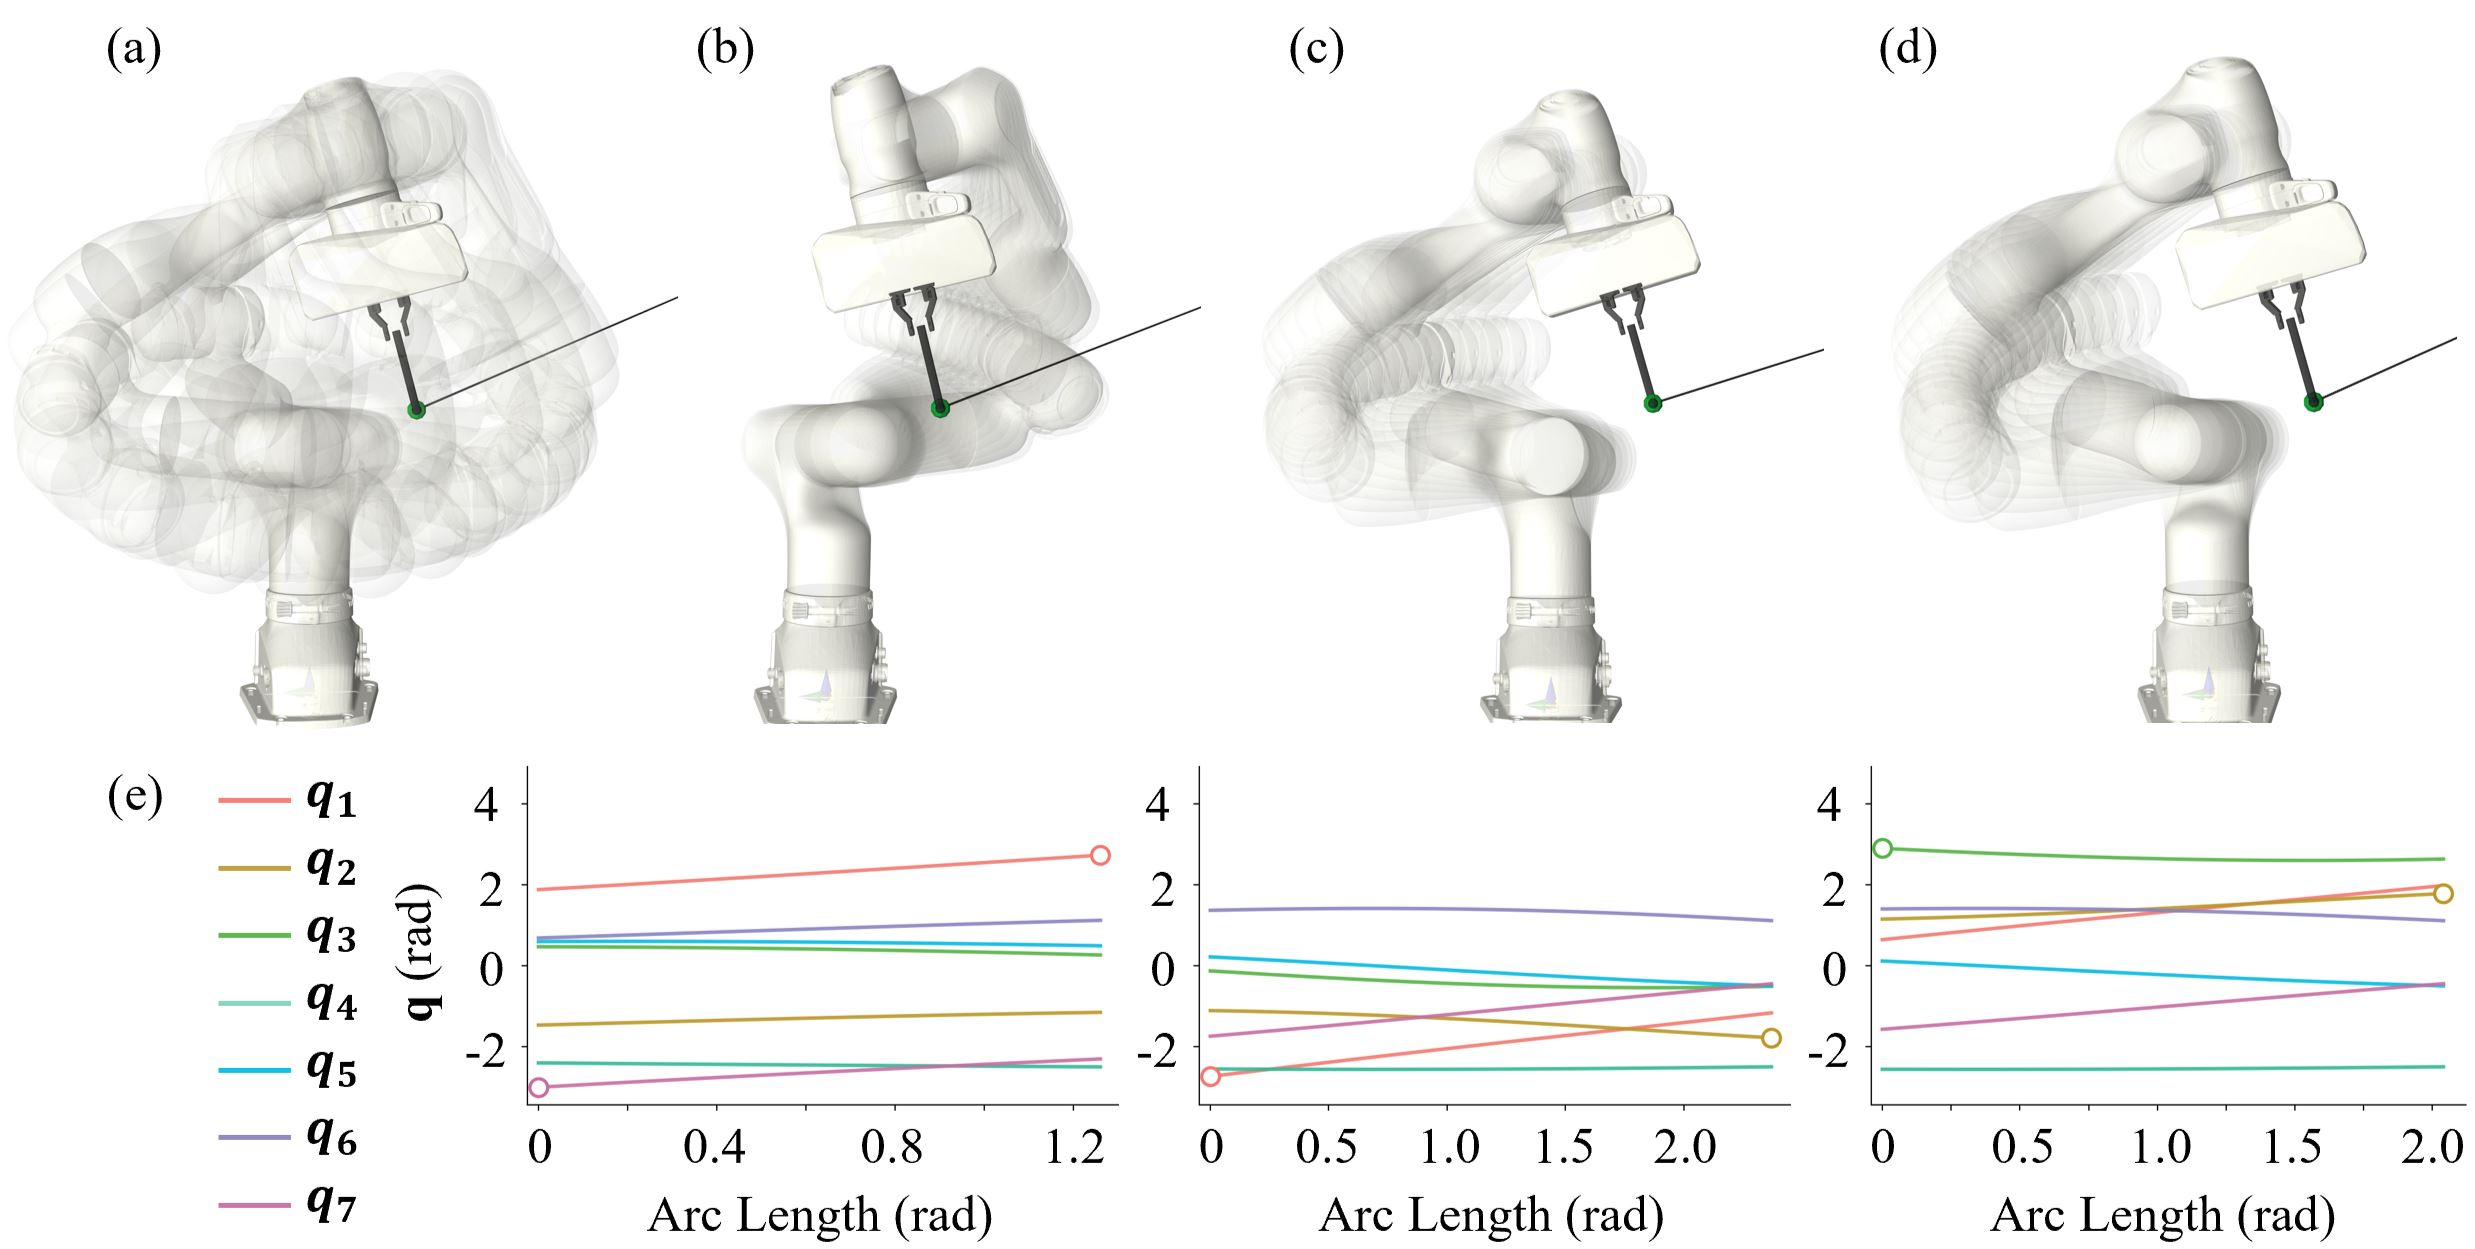
\includegraphics[width=\linewidth]{imgs/smm.JPG}
    \caption{Self-motion manifold for a fixed end-effector pose. (a) The continuous manifold without joint-limit constraints; (b)--(d) Configurations from the disconnected branches induced by the joint limits, sharing the same pose but differing sharply in joint space and reachable path length. (e) Joint trajectories of the three branches in b--d along the arc length, with circles marking the joint at its limit: branch~b bounded by $\mathbf{q}_{1}$ and $\mathbf{q}_{7}$, branch~c by $\mathbf{q}_{1}$, and $\mathbf{q}_{2}$ branch~d by $q_{2}$ and $\mathbf{q}_{3}$.}
    \label{smm}
\end{figure}

Therefore, this selection module aims to provide the hybrid controller with an initial joint configuration within a favorable branch. Consequently, the learned motion prior should incorporate configurations from various branches that yield a sufficient path length. For each task, we enumerate configurations across branches by cone-constrained IK solved by IKSel \cite{yuan2026iksel}, score each by a clean rollout under the classical controller, and retain the top-$K'$ scoring candidates ($K'{=}6$) that remain length-stable under small task perturbations as training labels.

The distribution of these initial joint configurations is approximated with a conditional DDPM~\cite{ho2020denoising}, where a residual-MLP denoiser generates a $7$-dimensional joint configuration $\mathbf{q}_{0}$ conditioned on the task vector $\mathbf{c}=[\mathbf{p}_{0};\mathbf{d};\mathbf{n}]$, trained under Classifier-Free Guidance (CFG) \cite{ho2022classifier} by dropping the condition with probability $p_{\mathrm{drop}}$. At inference, the guidance scale $w$ in
\begin{equation}
\label{eq:cfg}
\mathbf{v} = \mathbf{v}_{\theta}(\mathbf{x}_{t},t,\varnothing) + w\big(\mathbf{v}_{\theta}(\mathbf{x}_{t},t,\mathbf{c}) - \mathbf{v}_{\theta}(\mathbf{x}_{t},t,\varnothing)\big)
\end{equation}
controls the task signal, where $w=1$ recovers conditional sampling and $w>1$ amplifies it. \rev{At inference, we draw a batch of $K$ candidate configurations from this prior for each task and project each onto the exact position with the tool axis kept within the orientation cone, leaving the rotation about the tool axis free.}

\rev{Sampling the right distribution alone, however, does not determine the initial configuration: the candidates for a task land on different SMM branches whose reachable path lengths differ drastically, and while they are exchangeable in expectation---an arbitrarily chosen valid one performs no better than the per-task average---the best of the batch recovers substantially more of the reference length. The initialization is therefore a selection problem as much as a generation problem, and we select among the candidates with a learned scorer before the motion begins.}

\rev{We impose a strict deployment budget on this selection: no additional rollouts, and a single selection per task. Every candidate $\mathbf{q}_{0}^{(i)}$ is described by the same initial observation $\mathbf{o}_{0}$ that the policy receives (Eq.~\eqref{eq:obs}), augmented with the log directional manipulability, and a learned scorer $f_{\phi}$ predicts its achievable path length; the executed seed is $\mathbf{q}_{0}^{*}=\arg\max_{i} f_{\phi}(\mathbf{o}_{0}^{(i)})$. The configuration that generated the task is not available at deployment and is therefore excluded from the batch, and the scorer is a single multilayer perceptron. Its training data is obtained offline from the enumerated SMM candidates of each training task, scored once by the classical controller during the single labeling pass shared with the diffusion model and the policy. Because the scorer must pick the top candidate rather than predict lengths accurately, it is trained with a ranking objective; the choice among classical learning-to-rank objectives has little effect on the selected seed. The full selection at deployment consists of batched diffusion sampling, the per-candidate projection, and one forward pass of the scorer, with the scoring itself negligible in cost, so that a single candidate is chosen before the motion starts and executed by the learned controller without further intervention.}

\subsection{\xinyi{Student Policy:} RL-based Null-Space Controller}
\xinyi{The interior policy $\pi$ is trained with Proximal Policy Optimization (PPO). The observation $\mathbf{o}_{t}\in\mathbb{R}^{31}$ includes quantities that are related to redundancy resolution:
\begin{equation}
\label{eq:obs}
\mathbf{o}_{t}=\big[\,\bar{\mathbf{q}};\ \bar{\mathbf{q}}^{\odot 2};\ \mathbf{d};\ \mathbf{n};\ \mathbf{z}(\mathbf{q});\ \mathbf{z}(\mathbf{q})^{\top}\mathbf{n};\ \mathbf{z}(\mathbf{q})\times\mathbf{n};\ \mathbf{a}_{t-1}\,\big],
\end{equation}
where $\bar{\mathbf{q}}$ and $\bar{\mathbf{q}}^{\odot 2}$ are the normalized joint configuration and its element-wise square, $\mathbf{d}$ is the task direction along the pre-defined line, and $\mathbf{n}$ is the target normal of the task surface. The remaining terms characterize the tool axis $\mathbf{z}(\mathbf{q})$ relative to $\mathbf{n}$: the alignment $\mathbf{z}(\mathbf{q})^{\top}\mathbf{n}=\cos\theta$ measures how far the tool axis lies from the cone boundary, while the cross product $\mathbf{z}(\mathbf{q})\times\mathbf{n}$, with magnitude $\sin\theta$, encodes the direction of the orientation error. Finally, $\mathbf{a}_{t-1}$ denotes the previous action.}

The policy outputs a $4$-dimensional action $\mathbf{a}\in[-1,1]^{4}$ whose entries are coordinates in a task-aligned null-space basis $\mathbf{B}(\mathbf{q})\in\mathbb{R}^{7\times 4}$. The basis is constructed by Gram--Schmidt: the three projected gradients of the redundancy objectives in Eq.~\eqref{eq:secondary} are orthonormalized first, and the remaining one-dimensional orthogonal complement within the $4$-dimensional null space is appended to complete the basis. The resulting command $\dot{\mathbf{q}}_{\mathrm{null}}=\mathbf{B}(\mathbf{q})\,(\mathbf{a}_{\max})$ is added to the same task term as the classical controller in Eq.~\eqref{eq:nullspace}, so that the two regimes share one parameterization and are directly interchangeable at switching time.

Since the objective is simply to maximize the path length, the reward needs no elaborate shaping and is purely progress-based:
\begin{equation}
\label{eq:reward}
r_{t} = w_{p}\,\mathrm{clip}\!\left(\frac{(\mathbf{p}_{t+1}-\mathbf{p}_{t})^{\top}\mathbf{d}}{v\,\Delta t},\,0,\,1\right)\in[0,\,w_{p}],
\end{equation}
the per-step advance along $\mathbf{d}$ normalized by its maximum attainable value. No terminal penalty is imposed during the training process, and any violation directly terminates the episode.


\subsection{\xinyi{Teacher Policy: Hybrid Null-Space Controller}}\rev{\label{sec:coordination}}
\xinyi{Despite its strong performance, the trained student policy performs poorly near the joint-limit regions, where sparse data coverage leads to rapid and severe failures. We therefore introduce a model-based controller that takes over in this region, significantly increasing the roll-out path length. The model-based controller and RL-policy} are
combined at the level of individual control steps. 

\xinyi{In detail, the switching mechanism is based on the proximity to the joint limits, measured by the normalized joint-space distance}
\begin{equation}
\label{eq:rho}
\rho(\mathbf{q}) = \max_{i}\,\frac{|q_{i}-q_{\mathrm{mid},i}|}{(q_{\max,i}-q_{\min,i})/2}\in[0,1],
\end{equation}
which equals $0$ at the center of the joint range and $1$ at a limit. The RL policy governs the interior region, while the classical controller handles the near-boundary shell. To avoid chattering, the switching follows a hysteresis rule with two thresholds $\tau_{\mathrm{enter}}\ge\tau_{\mathrm{exit}}$: while the RL policy is active, control passes to the classical controller once $\rho\ge\tau_{\mathrm{enter}}$, and it returns to the RL policy only after $\rho$ falls back below $\tau_{\mathrm{exit}}$. If the initial configuration already lies in the boundary shell, i.e., $\rho(\mathbf{q}_{0}^{*})\ge\tau_{\mathrm{enter}}$, the episode begins under the classical controller. 
% \rev{For the distilled policy $\pi_{\mathrm{D}}$ of Section~\ref{sec:distill}, the thresholds are retuned on the evaluation protocol: a wide hysteresis gap $(\tau_{\mathrm{enter}},\tau_{\mathrm{exit}})=(0.985,0.96)$ preserves the path length while reducing switching to about $0.3$ transitions per episode, one quarter of the conference configuration.}


\rev{\subsection{\xinyi{Expert Iteration: Policy Self-Improvement}}\label{sec:distill}

Since the hybrid controller reliably attains a longer rollout length than the RL policy alone, a natural question is whether the RL policy can acquire this improved behavior by itself, so that the model-based controller becomes unnecessary at runtime. Two direct approaches are conceivable: optimizing the behavior within the reinforcement-learning framework, or fine-tuning the trained policy afterward. Neither succeeds in practice, for two reasons. First, exploration cannot discover the near-boundary behavior: in the boundary shell, a policy lacking this behavior terminates within a few steps, so the advantage estimates compare one short-lived trajectory against another and carry no usable gradient. Second, the behavior is not retained under further reinforcement learning: even when it is implanted by supervision, subsequent policy-gradient fine-tuning drifts back toward the on-policy objective and erodes it. The behavior itself is not hard to represent---a supervised fit of the classical secondary command from the observation of Eq.~\eqref{eq:obs} attains a coefficient of determination of $0.91$---so the obstacle lies in exploration and retention rather than in model capacity.

We therefore improve the policy through expert iteration. Rather than requiring the RL policy to discover the behavior on its own, we take the hybrid controller as an expert and distill it into a single student policy of the same architecture as the RL policy; the improved student then constitutes a stronger expert for the next round, closing the loop.

The learning target of each round is the expert policy $\pi^{*}$, constructed around the current student $\hat{\pi}$ as the hybrid null-space controller described above. When queried at a state, the expert returns the student's own action in the interior region, the classical controller's action in the boundary shell, and a linear blend of the two within a narrow band around the switching threshold; the blend removes the switching discontinuity that a smooth student network cannot represent. This construction, summarized in Algorithm~\ref{alg:expert}, requires only the two existing controllers and introduces no search, learned model, or additional hyperparameter.

The expert iteration then proceeds as in Algorithm~\ref{alg:exit}. In each round, the current student is rolled out in closed loop on the training tasks to collect the states it visits; the expert relabels these states, and the labels are aggregated with those of previous rounds in the manner of DAgger~\cite{ross2011reduction}, so that the student is corrected exactly on its own visitation distribution. The student is then refit to the aggregated labels by supervised regression, warm-started from its predecessor to preserve fidelity. Because the expert's interior branch is the student itself, an improved student yields a stronger expert, and the two improve together.

The loop is terminated by an improvement criterion: after each round we measure the fraction of tasks on which reinstating the runtime switch still lengthens the rollout beyond the student alone. This fraction decreases monotonically across rounds, indicating that the student progressively internalizes the boundary behavior; when it stabilizes, the expert no longer surpasses the student and the improvement operator is exhausted. The final policy $\pi_{\mathrm{D}}$ is taken as the parameter average of the last two students in the lineage~\cite{wortsman2022model}. The distilled policy then serves as the learning-based controller within the deployed framework.}

\begin{algorithm}[!htbp]
{\color{magenta}
\caption{Expert-iteration distillation of the hybrid controller.}
\label{alg:exit}
\KwIn{PPO-trained apprentice $\hat{\pi}_{0}$ (Sec.~IV-C); rounds $N$}
\KwOut{distilled policy $\pi_{\mathrm{D}}$}
$\pi^{*}_{0} \leftarrow \mathrm{BuildExpert}(\hat{\pi}_{0})$ \tcp*{Alg.~\ref{alg:expert}}
$\mathcal{D} \leftarrow \emptyset$\;
\For{$i \leftarrow 1$ \KwTo $N$}{
  $\mathcal{S}_{i} \leftarrow$ states visited by $\hat{\pi}_{i-1}$ in closed loop on training tasks\;
  $\mathcal{D}_{i} \leftarrow \{(\mathbf{s},\, \pi^{*}_{i-1}(\mathbf{s})) \mid \mathbf{s} \in \mathcal{S}_{i}\}$ \tcp*{expert labels}
  $\mathcal{D} \leftarrow \mathcal{D} \cup \mathcal{D}_{i}$ \tcp*{DAgger aggregation}
  $\hat{\pi}_{i} \leftarrow \arg\min_{\pi}\sum_{(\mathbf{s},\mathbf{a})\in\mathcal{D}}\|\pi(\mathbf{s})-\mathbf{a}\|^{2}$, initialized at $\hat{\pi}_{i-1}$\;
  $\pi^{*}_{i} \leftarrow \mathrm{BuildExpert}(\hat{\pi}_{i})$\;
  \If{the runtime switch no longer improves on $\hat{\pi}_{i}$}{
    \textbf{break} \tcp*{improvement operator exhausted}
  }
}
\Return $\pi_{\mathrm{D}} \leftarrow$ weight average of $\hat{\pi}_{N-1}$ and $\hat{\pi}_{N}$\;
}
\end{algorithm}

\begin{algorithm}[!htbp]
{\color{magenta}
\caption{BuildExpert: the hybrid behavior map, queried at state $\mathbf{s}$.}
\label{alg:expert}
\KwIn{apprentice $\hat{\pi}$; threshold $\tau$; band $b$}
\KwOut{expert action $\pi^{*}(\mathbf{s})$}
$\rho \leftarrow$ normalized joint-limit distance of $\mathbf{s}$, Eq.~\eqref{eq:rho}\;
\lIf{$\rho < \tau - b$}{\Return $\hat{\pi}(\mathbf{s})$ \tcp*[f]{interior: the apprentice}}
\lIf{$\rho \ge \tau$}{\Return $\mathbf{a}_{\mathrm{cls}}(\mathbf{s})$ \tcp*[f]{shell: the classical controller}}
$\lambda \leftarrow \big(\rho - (\tau - b)\big)/b$;\quad
\Return $(1-\lambda)\,\hat{\pi}(\mathbf{s}) + \lambda\,\mathbf{a}_{\mathrm{cls}}(\mathbf{s})$ \tcp*{band}
}
\end{algorithm}



%%%%%%%%%%%%%%%%%%%%%%%%%%%%%%%%%%%%%%%%%%%%%%%%%%%%%%%%%%%%%%%%%%%%%%%%%
\section{Experiments and Analysis}
\rev{\label{sec:exp}}
All experiments were conducted using the \textit{One} robotic system\footnote{https://github.com/wanweiwei07/one}, on the 7-DoF Franka Research 3 (FR3) with a pen-shaped tool attached to the end-effector. \rev{We sample $100{,}000$ collision-free straight-line path-following tasks within the FR3 work range, each specified by a starting position $\mathbf{p}_0$, a desired line direction $\mathbf{d}$, and a task-plane normal $\mathbf{n}$. The tasks are split once into a training set and a test set: we reserve $5{,}000$ tasks as a held-out test set that is frozen and never observed by any training component, and we run the self-motion-manifold labeling procedure on the remaining tasks and retain the $20{,}000$ qualified ones---those admitting at least one branch of sufficient reachable path length---as the training set. This single labeling pass supplies all three learned components: the qualified branches whose length lies within the top region serve as the diffusion training targets, the full set of candidates with their measured lengths serves as the ranking training data, and all enumerated branch configurations serve as the initial states for reinforcement learning. The reference length is computed only on the test set for evaluation and never enters training.}

Unless otherwise specified, experiments use the default setting: \rev{(1)} a diffusion-based initial configuration generator using DDIM with 50 denoising steps and CFG scale $w=1.5$; \rev{(2)} classical secondary-objective weights $k_{\mu},k_{\mathrm{jl}},k_{\theta}$ of $0.8,0.4,0.2$; \rev{(3) hybrid switching thresholds $\tau_{\mathrm{enter}},\tau_{\mathrm{exit}}$ of $0.985,0.96$; and (4) ranked initialization over a batch of diffusion candidates, from which the learned scorer selects the executed seed}.

\rev{For each test task, we generate candidate configurations following the same enumeration procedure and roll out every candidate under the classical controller. We denote the longest rollout length as the \emph{reference length} ($\ell^{\mathrm{ref}}$) and use it for the subsequent percentage comparison. As the reference is attained by a specific controller rather than a task-intrinsic bound, a configuration may exceed it, in which case the reported ratio surpasses $100\%$.}

\subsection{Results Analysis}
\subsubsection{Evaluation Set Analysis}
We partition the \rev{test} set into difficulty levels by the absolute reference length $\ell^{\mathrm{ref}}$: Easy ($\ell^{\mathrm{ref}}\ge 0.80$\,m, \rev{$n{=}0$}), Medium ($0.45\le\ell^{\mathrm{ref}}<0.80$\,m, \rev{$n{=}0$}), and Difficult ($\ell^{\mathrm{ref}}<0.45$\,m, \rev{$n{=}0$}). Intuitively, harder tasks exhibit a shorter best achievable path, reflected in a smaller reference length. Fig. \ref{fig:eval_dist} (a) shows the distribution of $\ell^{\mathrm{ref}}$ \rev{over the test set}.

\begin{figure}[!htbp]
    \centering
    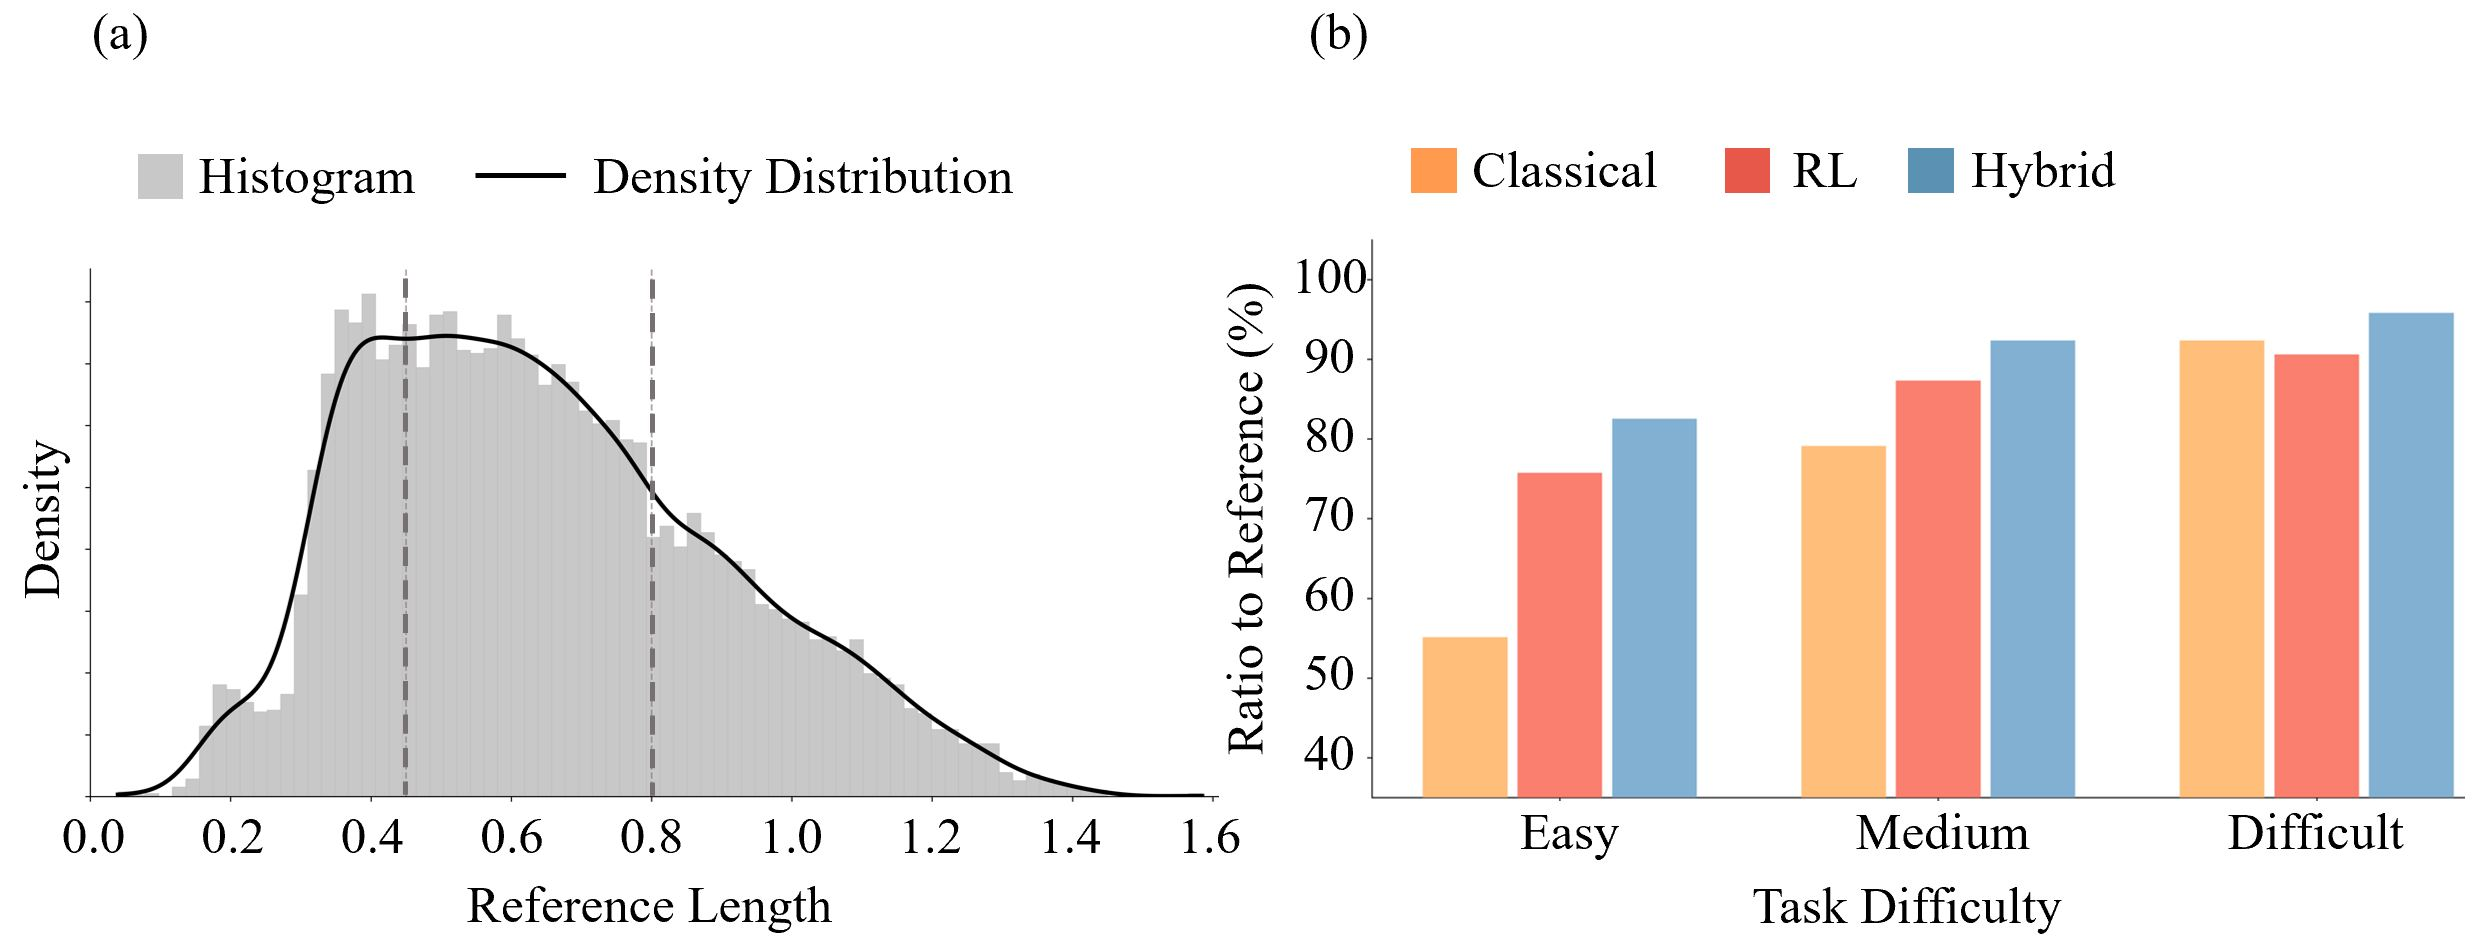
\includegraphics[width=\linewidth]{imgs/task_distribution.JPG}
    \caption{(a) Distribution of the reference length $\ell^{\mathrm{ref}}$ over the $10{,}000$ evaluation tasks. The dashed grey line marks the task-difficulty threshold.}
    \label{fig:eval_dist}
\end{figure}

\begin{figure}[!htbp]
    \centering
    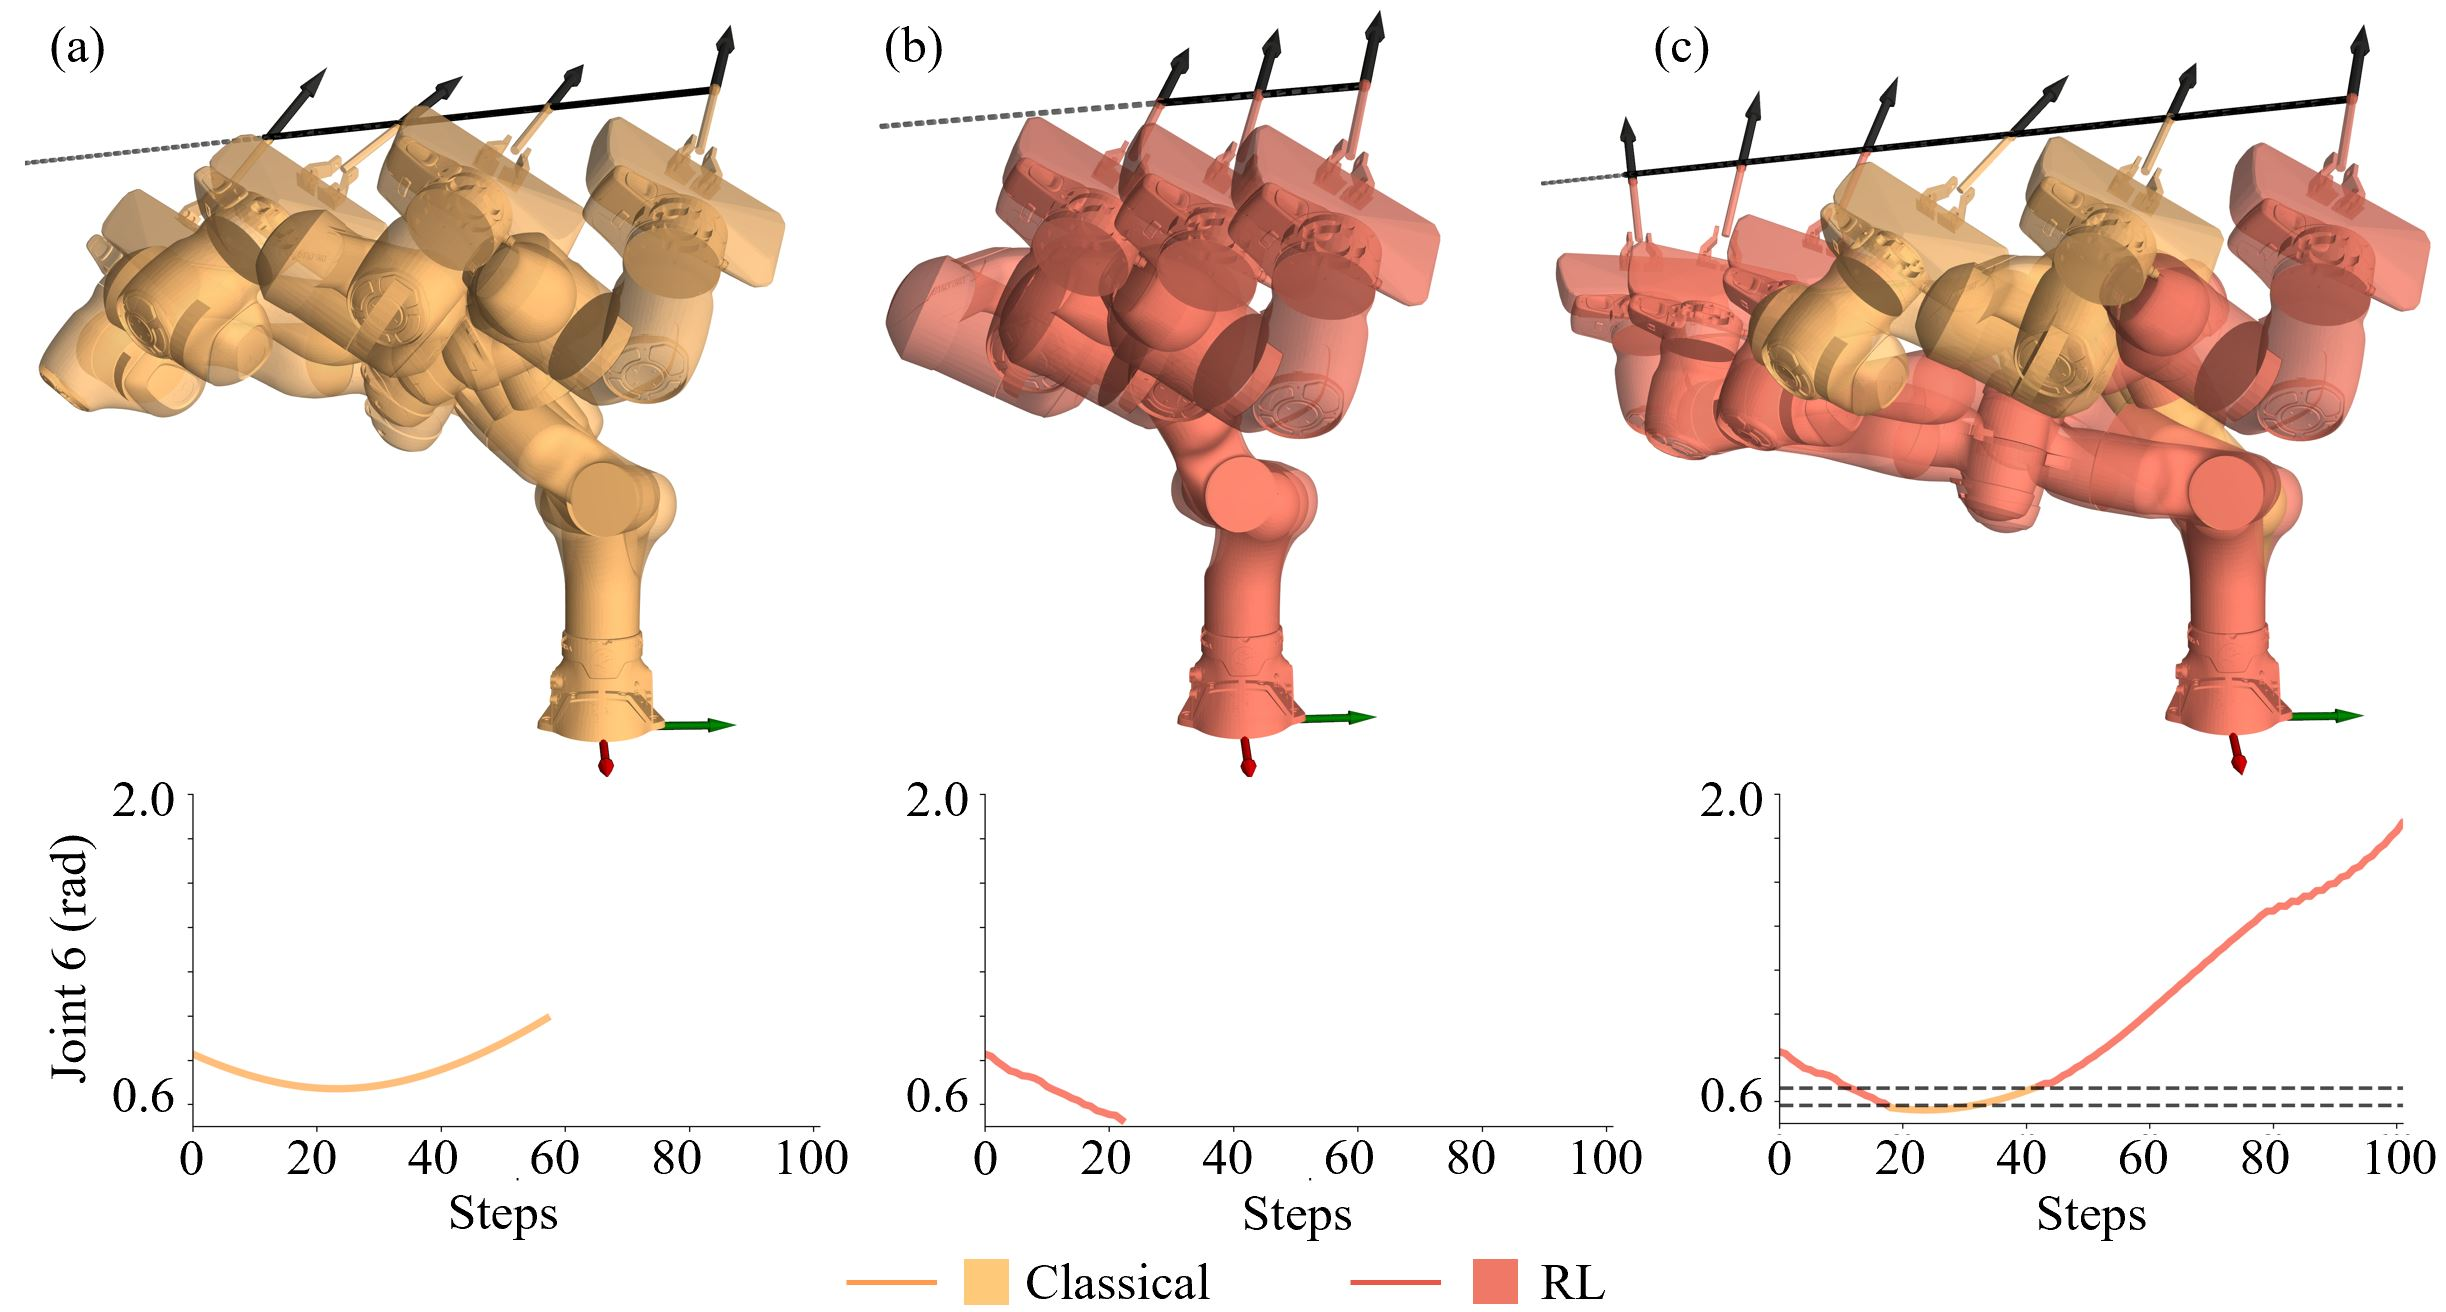
\includegraphics[width=\linewidth]{imgs/main_results.JPG}
    \caption{Qualitative comparison on a representative task: executed motion (top) and joint~6 trajectory (bottom), with color denoting the active controller. The dashed grey lines mark the $\tau_{\mathrm{enter}}/\tau_{\mathrm{exit}}$ thresholds mapped to the joint~6 limits.}
    \label{fig:main_result}
\end{figure}

\subsubsection{\xinyi{System Evaluation}}
\rev{This section reports the overall performance of the full system---the diffusion prior with ranked initialization together with the deployed controller---as a single method, and compares it against external baselines. The baseline comparison is left for a subsequent revision.}


\rev{\subsubsection{\xinyi{Expert Iteration Analysis}}\label{sec:distillresults}
Table~\ref{tab:distill} compares the controllers with the initial configuration fixed to the first IK-valid DP seed, and Fig.~\ref{fig:main_result} illustrates their behavior on a representative task. The reinforcement-learning policy exploits the interior margin well but its foresight advantage over the classical controller diminishes as the margin shrinks with task difficulty, matching classical parity on the Difficult bucket near the boundary; the hybrid controller attains the best of the three by delegating the near-boundary region to the classical controller. Two further observations concern the distilled policy $\pi_{\mathrm{D}}$. First, the standalone $\pi_{\mathrm{D}}$ surpasses the PPO policy and approaches the hybrid controller as a single network, confirming that the near-boundary behavior can be internalized without the model-based controller at runtime. Second, the difficulty gradient of the learned policy disappears: $\pi_{\mathrm{D}}$ is strongest exactly on the Difficult tasks, because the expert supplies, by imitation, precisely the near-boundary competence that reinforcement learning could not discover through exploration. Re-hosting $\pi_{\mathrm{D}}$ as the learning-based controller within the hybrid architecture retains only a small residual benefit from the runtime switch, so that the hybrid architecture is best understood as a policy-improvement operator whose value is largely distilled into a single network.}

\begin{table*}[!htbp]
\centering
\rev{
\caption{\rev{The Distilled Policy $\pi_{\mathrm{D}}$ against the Individual Controllers under the First IK-Valid DP Seed.}}
\label{tab:distill}
\begin{threeparttable}
\begin{tabular}{llcccc}
\toprule
Eval-Set & $\pi$
& \shortstack{Path Length (m)\\ {\scriptsize Mean / Std / Min / Max}}
& \shortstack{Ratio to Reference ($\%$)\\ {\scriptsize Mean / Std / Min / Max}} \\
\midrule
\multirow{5}{*}{\shortstack{All\\{\scriptsize \rev{($n{=}0$)}}}}
& \rev{Classical}                  & \rev{0 / 0 / 0 / 0} & \rev{0 / 0 / 0 / 0} \\
& RL                        & \rev{0 / 0 / 0 / 0} & \rev{0 / 0 / 0 / 0} \\
& $\pi_{\mathrm{D}}$ (distilled)      & \rev{0 / 0 / 0 / 0} & \rev{0 / 0 / 0 / 0} \\
& Hybrid                    & \rev{0 / 0 / 0 / 0} & \rev{0 / 0 / 0 / 0} \\
& Hybrid($\pi_{\mathrm{D}}$)          & \rev{0 / 0 / 0 / 0} & \rev{0 / 0 / 0 / 0} \\
\midrule
\multirow{5}{*}{\shortstack{Easy\\{\scriptsize \rev{($n{=}0$)}}}}
& \rev{Classical}                  & \rev{0 / 0 / 0 / 0} & \rev{0 / 0 / 0 / 0} \\
& RL                        & \rev{0 / 0 / 0 / 0} & \rev{0 / 0 / 0 / 0} \\
& $\pi_{\mathrm{D}}$ (distilled)      & \rev{0 / 0 / 0 / 0} & \rev{0 / 0 / 0 / 0} \\
& Hybrid                    & \rev{0 / 0 / 0 / 0} & \rev{0 / 0 / 0 / 0} \\
& Hybrid($\pi_{\mathrm{D}}$)          & \rev{0 / 0 / 0 / 0} & \rev{0 / 0 / 0 / 0} \\
\midrule
\multirow{5}{*}{\shortstack{Medium\\{\scriptsize \rev{($n{=}0$)}}}}
& \rev{Classical}                  & \rev{0 / 0 / 0 / 0} & \rev{0 / 0 / 0 / 0} \\
& RL                        & \rev{0 / 0 / 0 / 0} & \rev{0 / 0 / 0 / 0} \\
& $\pi_{\mathrm{D}}$ (distilled)      & \rev{0 / 0 / 0 / 0} & \rev{0 / 0 / 0 / 0} \\
& Hybrid                    & \rev{0 / 0 / 0 / 0} & \rev{0 / 0 / 0 / 0} \\
& Hybrid($\pi_{\mathrm{D}}$)          & \rev{0 / 0 / 0 / 0} & \rev{0 / 0 / 0 / 0} \\
\midrule
\multirow{5}{*}{\shortstack{Difficult\\{\scriptsize \rev{($n{=}0$)}}}}
& \rev{Classical}                  & \rev{0 / 0 / 0 / 0} & \rev{0 / 0 / 0 / 0} \\
& RL                        & \rev{0 / 0 / 0 / 0} & \rev{0 / 0 / 0 / 0} \\
& $\pi_{\mathrm{D}}$ (distilled)      & \rev{0 / 0 / 0 / 0} & \rev{0 / 0 / 0 / 0} \\
& Hybrid                    & \rev{0 / 0 / 0 / 0} & \rev{0 / 0 / 0 / 0} \\
& Hybrid($\pi_{\mathrm{D}}$)          & \rev{0 / 0 / 0 / 0} & \rev{0 / 0 / 0 / 0} \\
\bottomrule
\end{tabular}
\begin{tablenotes}
    \item[Note 1] \rev{All rows use the first IK-valid DP seed. Hybrid uses the RL policy as its learning-based controller, whereas Hybrid($\pi_{\mathrm{D}}$) uses the distilled policy.}
\end{tablenotes}
\end{threeparttable}}
\end{table*}

\subsubsection{Initial Configuration Selection}
\rev{This part analyzes the initialization stage in three aspects: the diffusion-based generation of candidate configurations, the learned selection among them, and the distribution shift between the enumeration data used to train the selection and the diffusion data seen at deployment.}

\rev{\emph{Diffusion-based generation.}}
Table~\ref{tab:seedsel} isolates the seed-selection module by fixing the controller and varying $\mathbf{q}_{0}^{*}$ across three sources: a manipulability seed, a joint-limit-centering seed, and the proposed DP seed. The two heuristics share one procedure, differing only in objective: null-space gradient ascent from $\mathbf{q}_{0}^{\mathrm{seed}}$ with periodic Newton re-projection onto the exact pose. As the ascent stays within the null space, both remain confined to the SMM branch of $\mathbf{q}_{0}^{\mathrm{seed}}$ and cannot cross to another, whereas DP samples a multi-modal distribution spanning multiple branches. \rev{Under every controller, DP leads both heuristics at comparable seed-generation cost, confirming that the learned prior reaches a more favorable starting branch than branch-bound heuristic refinement.} Fig.~\ref{fig:diversity} visualizes the multi-modal seeds the diffusion model samples on a representative task.

\rev{\emph{Learned selection.} Because the diffusion samples for a task land on different branches whose reachable lengths differ, the initialization is a selection problem rather than a single-sample generation. Table~\ref{tab:ranked} reports the full method, in which the learned scorer selects one candidate from the sampled batch before execution: ranked selection lifts the deployed system over the first-valid baseline toward the best-of-batch bound, recovering most of the selection headroom without rolling out any candidate. We further compare several classical learning-to-rank objectives for the scorer in Table~\ref{tab:progression}; the choice of objective has little effect, indicating that the selected seed need not be optimal but only needs to lie within the top region of the batch.}

\rev{\emph{Distribution shift and fine-tuning.} The scorer is trained on the enumerated SMM candidates, scored by the classical controller during the single labeling pass, whereas at deployment it ranks diffusion samples that are subsequently executed by the learned controller. This introduces a shift between the training and deployment distributions, both in the candidate source (enumerated versus diffusion samples) and in the controller that determines the achievable length (classical versus learned). We therefore examine whether an additional fine-tuning stage, which re-scores the diffusion candidates under the deployed controller, is necessary to close this shift.}

\begin{figure}[!htbp]
    \centering
    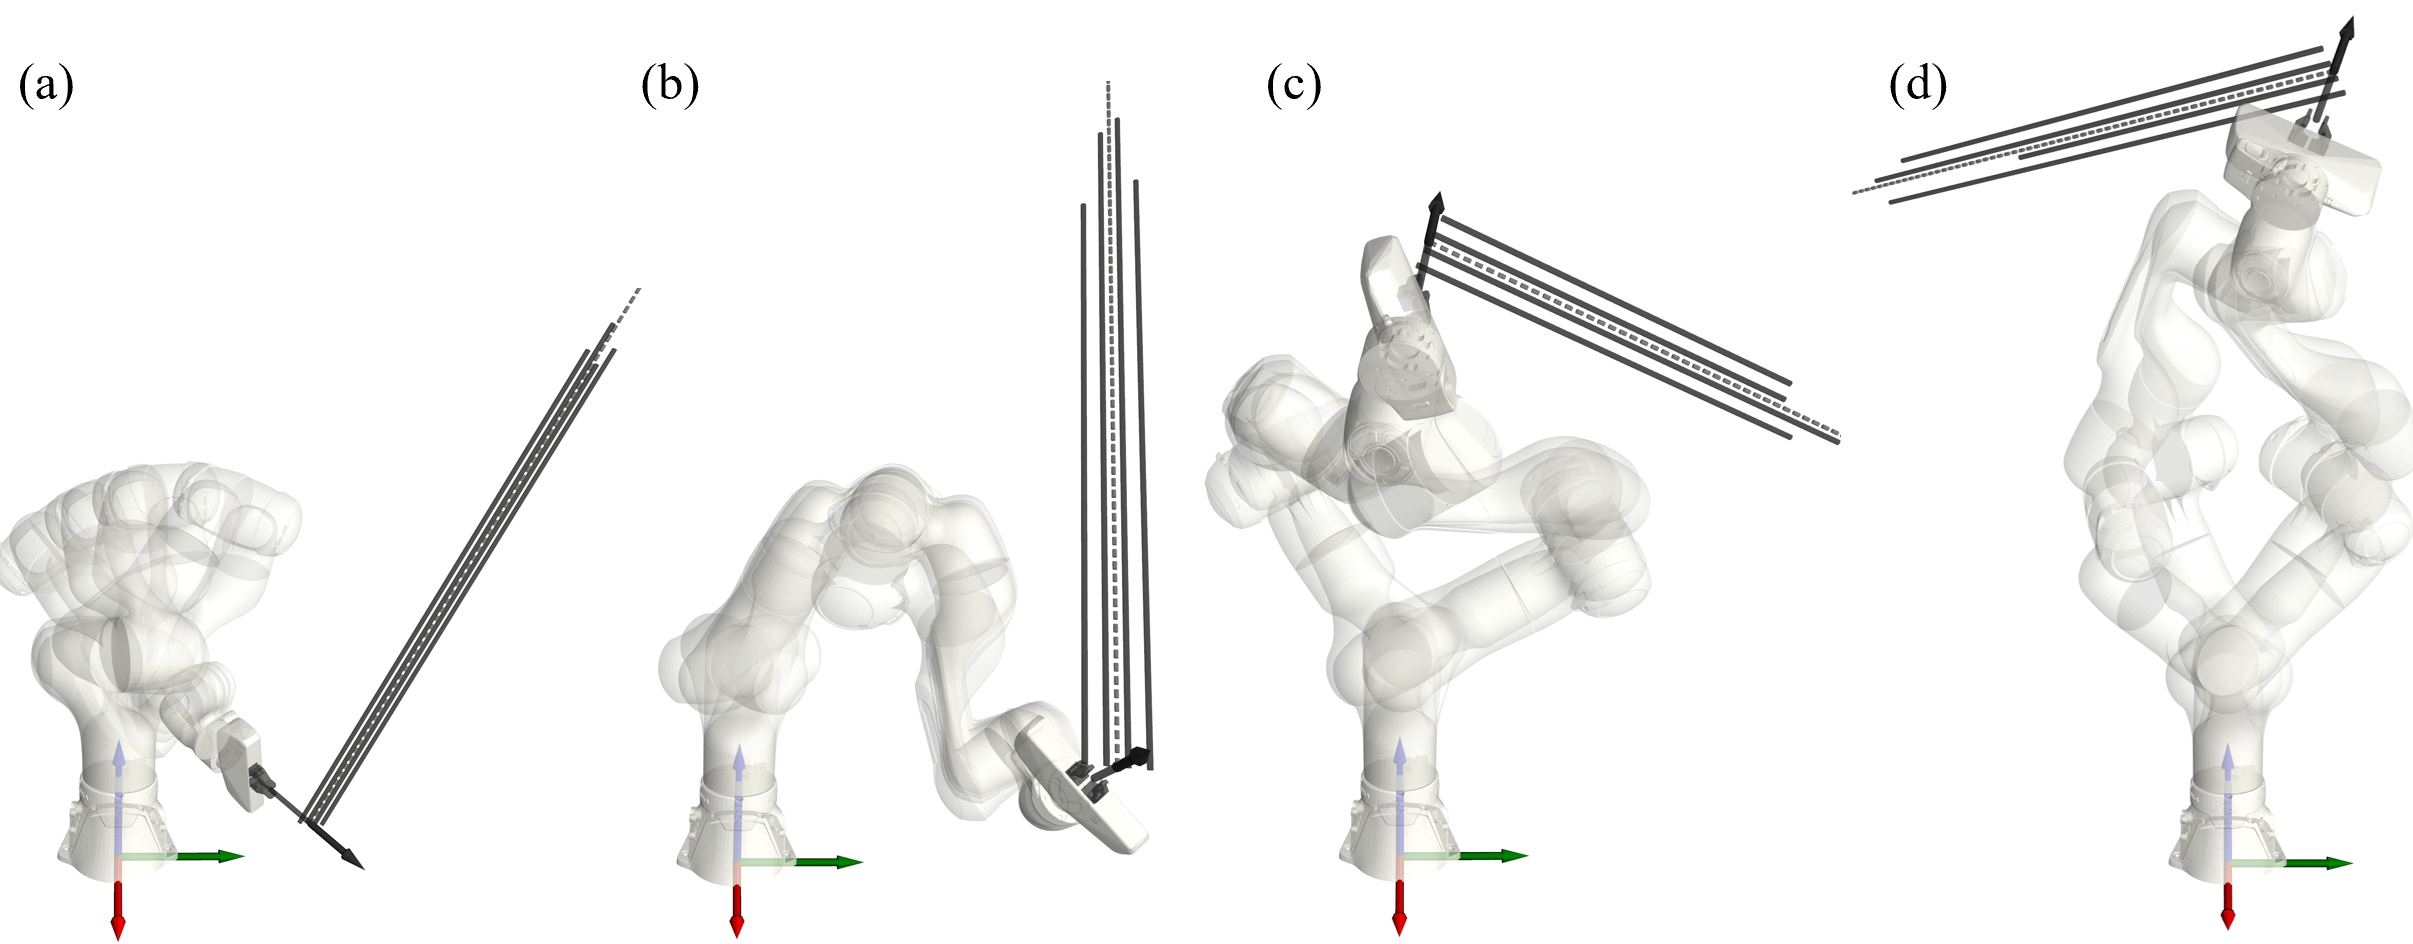
\includegraphics[width=\linewidth]{imgs/diversity.JPG}
    \caption{Multi-modal initial configurations sampled by the diffusion model. The dashed grey line denotes the actual motion direction, while the solid lines are laterally offset for clearer visualization.}
    \label{fig:diversity}
\end{figure}



\begin{table*}[!htbp]
\centering
% \setlength{\tabcolsep}{6pt}
\caption{Performance of the Proposed Initial Configuration Selection Method Compared with Heuristic Designs.}
\label{tab:seedsel}
\begin{threeparttable}
\begin{tabular}{llccc}
\toprule
$\pi$ & $\textbf{q}_{0}^*$ 
& $t$ (ms)
& \shortstack{Path Length (m)\\ {\scriptsize Mean / Std / Min / Max}} 
& \shortstack{Ratio to Reference ($\%$)\\ {\scriptsize Mean / Std / Min / Max}} \\
\midrule
\multirow{3}{*}{Classical}
& $\mathbf{q}_{\mu}$         & \rev{0} & \rev{0 / 0 / 0 / 0} & \rev{0 / 0 / 0 / 0} \\
& $\mathbf{q}_{\mathrm{jl}}$  & \rev{0} & \rev{0 / 0 / 0 / 0} & \rev{0 / 0 / 0 / 0} \\
& DP           & \rev{0} & \rev{0 / 0 / 0 / 0} & \rev{0 / 0 / 0 / 0} \\
\midrule
\multirow{3}{*}{RL}
& $\mathbf{q}_{\mu}$ & \rev{0} & \rev{0 / 0 / 0 / 0} & \rev{0 / 0 / 0 / 0} \\
& $\mathbf{q}_{\mathrm{jl}}$              & \rev{0} & \rev{0 / 0 / 0 / 0} & \rev{0 / 0 / 0 / 0} \\
& DP             & \rev{0} & \rev{0 / 0 / 0 / 0} & \rev{0 / 0 / 0 / 0} \\
\midrule
\multirow{3}{*}{Hybrid}
& $\mathbf{q}_{\mu}$         & \rev{0} & \rev{0 / 0 / 0 / 0} & \rev{0 / 0 / 0 / 0} \\
& $\mathbf{q}_{\mathrm{jl}}$  & \rev{0} & \rev{0 / 0 / 0 / 0} & \rev{0 / 0 / 0 / 0} \\
& DP           & \rev{0} & \rev{0 / 0 / 0 / 0} & \rev{0 / 0 / 0 / 0} \\
\bottomrule
\end{tabular}
\begin{tablenotes}
    \item[Note 1] $t$ is per-task seed-generation time.
    \item[Note 2] $\mathbf{q}_{\mu}$: manipulability-maximizing seed; $\mathbf{q}_{\mathrm{jl}}$: joint-limit-centering seed.
\end{tablenotes}
\end{threeparttable}
\end{table*}






\begin{table*}[!htbp]
\centering
\rev{
\caption{\rev{Ranked Initialization: the Full Method and the Selection Headroom on the Test Set.}}
\label{tab:ranked}
\begin{threeparttable}
\begin{tabular}{llcc}
\toprule
Eval-Set & Initialization ($\pi=$ Hybrid($\pi_{\mathrm{D}}$))
& \shortstack{Path Length (m)\\ {\scriptsize Mean / Std / Min / Max}}
& \shortstack{Ratio to Reference ($\%$)\\ {\scriptsize Mean / Std / Min / Max}} \\
\midrule
\multirow{3}{*}{\shortstack{All\\{\scriptsize \rev{($n{=}0$)}}}}
& First IK-valid  & \rev{0 / 0 / 0 / 0} & \rev{0 / 0 / 0 / 0} \\
& Ranked & \rev{0 / 0 / 0 / 0} & \rev{0 / 0 / 0 / 0} \\
& \textit{Best-of-batch (oracle)} & \rev{\textit{0}} & \rev{\textit{0}} \\
\midrule
\multirow{2}{*}{\shortstack{Easy\\{\scriptsize \rev{($n{=}0$)}}}}
& First IK-valid  & \rev{0 / 0 / 0 / 0} & \rev{0 / 0 / 0 / 0} \\
& Ranked & \rev{0 / 0 / 0 / 0} & \rev{0 / 0 / 0 / 0} \\
\midrule
\multirow{2}{*}{\shortstack{Medium\\{\scriptsize \rev{($n{=}0$)}}}}
& First IK-valid  & \rev{0 / 0 / 0 / 0} & \rev{0 / 0 / 0 / 0} \\
& Ranked & \rev{0 / 0 / 0 / 0} & \rev{0 / 0 / 0 / 0} \\
\midrule
\multirow{2}{*}{\shortstack{Difficult\\{\scriptsize \rev{($n{=}0$)}}}}
& First IK-valid  & \rev{0 / 0 / 0 / 0} & \rev{0 / 0 / 0 / 0} \\
& Ranked & \rev{0 / 0 / 0 / 0} & \rev{0 / 0 / 0 / 0} \\
\bottomrule
\end{tabular}
\begin{tablenotes}
    \item[Note 1] \rev{Best-of-$K$ oracle prefixes over the $w{=}1.5$ candidates: $K{=}2$: $0\%$, $K{=}4$: $0\%$, $K{=}8$: $0\%$; mean over valid candidates: $0\%$ ($\approx$ first-valid, i.e., candidates are exchangeable).}
    \item[Note 2] \rev{Selection cost: $0$\,s/task (batched DDIM $+$ Newton projections $+$ one scorer forward pass). No rollout is performed at deployment.}
\end{tablenotes}
\end{threeparttable}}
\end{table*}

\begin{table}[!htbp]
\centering
\rev{
\caption{\rev{Ablations of Ranked Initialization.}\xinyitodo{需要列举出来对比的ranking method}}
\label{tab:progression}
\begin{threeparttable}
\begin{tabular}{lc}
\toprule
\rev{Ranking objective} & Ratio to Ref.\ ($\%$) \\
\midrule
\rev{First IK-valid (no selection)}                 & \rev{0} \\
\midrule
\rev{Pointwise regression}                          & \rev{0} \\
\rev{RankNet (pairwise)~\cite{burges2005learning}}  & \rev{0} \\
\rev{ListNet (listwise)~\cite{cao2007learning}}     & \rev{0} \\
\rev{ListMLE (listwise)~\cite{xia2008listwise}}     & \rev{0} \\
\rev{LambdaRank~\cite{burges2010ranknet}}           & \rev{0} \\
\rev{Contrastive (adopted)~\cite{khosla2020supervised}} & \rev{\limebox{0}} \\
\midrule
\rev{\textit{Best-of-batch (oracle)}}               & \rev{\textit{0}} \\
\bottomrule
\end{tabular}
\begin{tablenotes}
    \item[Note 1] \rev{All rows share the same candidate batch, features, and the deployed controller Hybrid($\pi_{\mathrm{D}}$); they differ only in the ranking objective. The choice of ranking objective has little effect: the seed need not be optimal, only within the top region.}
\end{tablenotes}
\end{threeparttable}}
\end{table}

\subsection{Ablation Study}

Unless otherwise specified, each ablation study uses the diffusion-based initial configuration under the hybrid controller with the default parameters introduced at the beginning of the experiment section.

\subsubsection{Classical Null-Space Controller Hyperparameters}

Table~\ref{tab:ablate_classical} isolates the three secondary objectives of Eq.~\eqref{eq:secondary} and then sweeps their weighted combination.  The full sweep covers a $4\times3\times3$ grid of $(k_{\mu},k_{\mathrm{jl}},k_{\theta})$ plus three single-objective settings ($39$ in total), of which the table lists a representative subset. We use the task's generating configuration $\mathbf{q}_{0}^{\mathrm{seed}}$ as the initialization for simplicity. The first three rows activate one objective at a time (gain $1.0$); the next rows increase $k_{\mu}$ at near-fixed $k_{\mathrm{jl}}$. Single objectives are uniformly weak ($58.7$--$62.3\%$), and any mixed combination surpasses them, indicating that the secondary objectives are complementary rather than redundant. Nonetheless, while tuned mixed-weight settings may help on individual tasks, no combination yields a meaningful improvement across the full evaluation set.

\begin{table*}[!htbp]
\centering
% \setlength{\tabcolsep}{8pt}
\caption{Ablation of the Classical Secondary-Objective Weights.}
\label{tab:ablate_classical}
\begin{threeparttable}
\begin{tabular}{ccccc}
\toprule
$k_{\mu}$ & $k_{\mathrm{jl}}$ & $k_{\theta}$
& \shortstack{Path Length (m)\\ {\scriptsize Mean / Std / Min / Max}}
& \shortstack{Ratio to Reference ($\%$)\\ {\scriptsize Mean / Std / Min / Max}} \\
\midrule
1.0 & ---        & ---        & 0.36 / 0.15 / 0.01 / 1.15 & 62.3 / 29.5 / 0.8 / 1027.8 \\
---        & \pinkbox{1.0} & ---        & \pinkbox{0.34} / 0.17 / 0.02 / 1.28 & \pinkbox{58.7} / 28.5 / 3.5 / \phantom{0}521.9 \\
---        & ---        & 1.0 & 0.35 / 0.13 / 0.01 / 1.14 & 60.6 / 28.0 / 0.9 / \phantom{0}945.8 \\
\midrule
0.2 & 0.1 & 0.4 & 0.36 / 0.13 / 0.01 / 1.12 & 62.6 / 26.6 / 1.9 / \phantom{0}675.8 \\
0.4 & 0.2 & 0.4 & 0.37 / 0.14 / 0.02 / 1.16 & 63.7 / 26.7 / 2.5 / \phantom{0}675.9 \\
0.6 & 0.2 & 0.4 & 0.37 / 0.14 / 0.03 / 1.17 & 64.2 / 28.4 / 3.7 / \phantom{0}985.9 \\
0.8 & 0.2 & 0.4 & 0.37 / 0.15 / 0.03 / 1.17 & \limebox{64.5} / 28.8 / 3.2 / \phantom{0}986.3 \\
0.8 & 0.4 & 0.2 & 0.37 / 0.15 / 0.04 / 1.14 & 64.2 / 27.1 / 7.0 / \phantom{0}651.0 \\
\bottomrule
\end{tabular}
\begin{tablenotes}
    \item[Note 1] The cone gate $g(\theta)$ is rarely activated due to the conservativeness of the classical controller, so varying $k_{\theta}$ has little effect on performance.
\end{tablenotes}
\end{threeparttable}
\end{table*}

\subsubsection{Classifier-Free Guidance Scale}

Table~\ref{tab:ablate_cfg} varies the guidance scale $w$ of Eq.~\eqref{eq:cfg}, where $w=0$ ignores the task condition and larger $w$ amplifies it. The results show that performance peaks at $w=1.5$ ($90.6\%$), degrading under both unconditional sampling ($w=0$, $80.8\%$) and over-guidance ($w=3.0$, $84.2\%$). The seed-generation time $t$ is likewise lowest near $w=1.5$ and rises sharply at both ends ($133$\,ms at $w=0$, $94$\,ms at $w=3.0$, versus $\sim$46\,ms), as poorly conditioned samples need more sampling-and-projection retries to reach an IK-valid pose.

\begin{table*}[!htbp]
\centering
% \setlength{\tabcolsep}{8pt}
\caption{Effect of the Guidance Scale $w$ on Path Length and Seed-Generation Cost.}
\label{tab:ablate_cfg}
\begin{threeparttable}
\begin{tabular}{lccc}
\toprule
$w$
& $t$ (ms)
& \shortstack{Path Length (m)\\ {\scriptsize Mean / Std / Min / Max}}
& \shortstack{Ratio to Reference ($\%$)\\ {\scriptsize Mean / Std / Min / Max}} \\
\midrule
0.0 & \pinkbox{133.50} & \pinkbox{0.50} / 0.25 / 0.01 / 1.49 & \pinkbox{80.8} / 29.3 / 0.8 / \phantom{0}566.5 \\
1.0 & \phantom{0}46.90 & 0.56 / 0.25 / 0.01 / 1.48 & 89.4 / 22.9 / 0.7 / \phantom{0}562.7 \\
1.5 & \phantom{0}\limebox{46.40} & \limebox{0.57} / 0.25 / 0.01 / 1.45 & \limebox{90.6} / 23.1 / 0.8 / 1000.8 \\
2.0 & \phantom{0}50.20 & 0.56 / 0.25 / 0.01 / 1.45 & 89.5 / 23.3 / 0.8 / \phantom{0}666.4 \\
3.0 & \phantom{0}94.00 & 0.52 / 0.24 / 0.01 / 1.40 & 84.2 / 26.2 / 0.8 / \phantom{0}506.0 \\
\bottomrule
\end{tabular}
\end{threeparttable}
\end{table*}

\subsubsection{Number of Diffusion Sampling Steps}

Table~\ref{tab:ablate_steps} examines the influence of the DDIM sampling steps on both time cost and seed quality. The results indicate that both metrics remain flat across the step range $10$--$100$. We therefore conclude that the result is essentially insensitive to the number of sampling steps, and we adopt $50$ as the default. The underlying reason may be that the seed quality is retained within a few denoising steps, as it largely depends on the SMM branch. Moreover, regarding time cost, although more sampling steps increase the sampling time, the dominant bottleneck of seed generation is the number of re-projection retries, which also depends on the seed quality.

\begin{table*}[!htbp]
\centering
% \setlength{\tabcolsep}{6pt}
\caption{Effect of the DDIM Sampling Steps on Seed Quality and Time Cost.}
\label{tab:ablate_steps}
\begin{threeparttable}
\begin{tabular}{lccc}
\toprule
DDIM Steps
& $t$ (ms)
& \shortstack{Path Length (m)\\ {\scriptsize Mean / Std / Min / Max}}
& \shortstack{Ratio to Reference ($\%$)\\ {\scriptsize Mean / Std / Min / Max}} \\
\midrule
\phantom{0}10  & \pinkbox{48.80} & \limebox{0.572} / 0.245 / 0.010 / 1.448 & \limebox{90.6} / 20.9 / 0.9 / \phantom{0}659.0 \\
\phantom{0}20  & \limebox{46.40} & 0.570 / 0.244 / 0.010 / 1.487 & 90.5 / 22.1 / 0.8 / \phantom{0}683.3 \\
\phantom{0}50  & 46.50 & 0.571 / 0.246 / 0.010 / 1.448 & 90.6 / 23.1 / 0.8 / 1000.8 \\
100 & 47.30 & \pinkbox{0.569} / 0.247 / 0.010 / 1.590 & \pinkbox{90.2} / 21.9 / 0.8 / \phantom{0}567.4 \\
\bottomrule
\end{tabular}
\end{threeparttable}
\end{table*}



\subsubsection{Hybrid Switching Hyperparameters}

Table~\ref{tab:ablate_switch} varies the switching thresholds of Eq.~\eqref{eq:rho}. The top rows sweep a single threshold $\tau_{\mathrm{enter}}=\tau_{\mathrm{exit}}\in\{0.85,0.90,0.95,\\0.97,0.98,0.99\}$, tracing the performance comparison as the boundary region widens or shrinks. The bottom rows, in contrast, introduce a hysteresis gap with $\tau_{\mathrm{enter}}>\tau_{\mathrm{exit}}$, and the \emph{switches} column reports the mean number of transitions per episode. Results show that introducing the hysteresis gap largely reduces the number of switches compared with the single-threshold setting. We therefore adopt $(0.98,0.94)$ as the default, as it achieves a balanced performance between path-following length and switching stability.


\begin{table*}[!htbp]
\centering
% \setlength{\tabcolsep}{4.8pt}
\caption{Ablation of the Switching Thresholds $(\tau_{\mathrm{enter}},\tau_{\mathrm{exit}})$.}
\label{tab:ablate_switch}
\begin{threeparttable}
\begin{tabular}{lccc}
\toprule
$(\tau_{\mathrm{enter}},\tau_{\mathrm{exit}})$
& \shortstack{Switches\\ {\scriptsize Mean / Episode}}
& \shortstack{Path Length (m)\\ {\scriptsize Mean / Std / Min / Max}}
& \shortstack{Ratio to Reference ($\%$)\\ {\scriptsize Mean / Std / Min / Max}} \\
\midrule
$(0.85,\,0.85)$ & \pinkbox{2.50} & \pinkbox{0.534} / 0.231 / 0.010 / 1.427 & \pinkbox{86.1} / 24.3 / 0.8 / \phantom{0}601.3 \\
$(0.90,\,0.90)$ & 2.49 & 0.556 / 0.239 / 0.010 / 1.437 & 88.8 / 22.9 / 0.8 / \phantom{0}601.3 \\
$(0.95,\,0.95)$ & 1.97 & 0.571 / 0.244 / 0.010 / 1.437 & 90.7 / 23.7 / 0.8 / 1001.2 \\
$(0.97,\,0.97)$ & 1.65 & \limebox{0.573} / 0.246 / 0.010 / 1.448 & \limebox{90.9} / 23.1 / 0.8 / 1001.9 \\
$(0.98,\,0.98)$ & 1.43 & 0.572 / 0.247 / 0.010 / 1.448 & 90.7 / 22.7 / 0.8 / 1002.2 \\
$(0.99,\,0.99)$ & 0.99 & 0.563 / 0.253 / 0.010 / 1.448 & 89.3 / 24.8 / 0.8 / 1017.6 \\
\midrule
$(0.98,\,0.94)$ & 0.44 & 0.571 / 0.246 / 0.010 / 1.448 & 90.6 / 23.1 / 0.8 / 1000.8 \\
$(0.99,\,0.93)$ & \limebox{0.32} & 0.567 / 0.247 / 0.010 / 1.448 & 90.0 / 23.9 / 0.8 / 1017.6 \\
\bottomrule
\end{tabular}
\begin{tablenotes}
    \item[Note 1] Only representative swept hysteresis combinations are listed.
\end{tablenotes}
\end{threeparttable}
\end{table*}

\rev{\subsubsection{Expert Iteration Convergence}
Table~\ref{tab:ablate_exit} traces the expert iteration round by round. Round $0$ is the PPO policy; each subsequent round rebuilds the expert around the current student and distills it. Two quantities are reported: the ratio to reference of the standalone student, and the fraction of tasks on which reinstating the runtime switch still lengthens the rollout beyond the student alone, which serves as the improvement criterion. The standalone student improves monotonically while the switch-benefit fraction decreases, indicating that the boundary behavior is progressively internalized; once the fraction stabilizes, the expert no longer surpasses the student and the loop is terminated.}

\begin{table}[!htbp]
\centering
\rev{
\caption{\rev{Convergence of Expert Iteration over Rounds.}}
\label{tab:ablate_exit}
\begin{threeparttable}
\begin{tabular}{lcc}
\toprule
Round & \shortstack{Standalone $\hat{\pi}_{i}$\\ Ratio to Ref.\ ($\%$)} & \shortstack{Switch-benefit\\ Fraction ($\%$)} \\
\midrule
$0$ (PPO)          & $0$ & $0$ \\
$1$                & $0$ & $0$ \\
$2$                & $0$ & $0$ \\
$3$                & $0$ & $0$ \\
$4$                & $0$ & $0$ \\
$\cdots$           & $\cdots$ & $\cdots$ \\
$N-1$              & $0$ & $0$ \\
$N$                & $0$ & $0$ \\
\midrule
$\pi_{\mathrm{D}}$ (averaged) & \limebox{$0$} & $0$ \\
\bottomrule
\end{tabular}
\begin{tablenotes}
    \item[Note 1] $\pi_{\mathrm{D}}$ is the parameter average of the last two students.
\end{tablenotes}
\end{threeparttable}}
\end{table}

%%%%%%%%%%%%%%%%%%%%%%%%%%%%%%%%%%%%%%%%%%%%%%%%%%%%%%%%%%%%%%%%%%%%%%
\section{Conclusions and Future Work}
\label{sec:conclusion}
%%%%%%%%%%%%%%%%%%%%%%%%%%%%%%%%%%%%%%%%%%%%%%%%%%%%%%%%%%%%%%%%%%%%%%

In this paper, we developed a framework for extreme motion generation that advances a fixed-base manipulator along a prescribed straight line as far as possible. The framework adopts a step-level hybrid null-space controller, which delegates the well-sampled interior to an RL policy for length maximization and the near-boundary region to a robust classical controller through a hysteresis switching rule. Prior to execution, a conditional diffusion model initializes the manipulator on a favorable branch of the SMM. Experimental results demonstrated a longer path-following length than both the classical and learning-based controllers and showed that the hysteresis switching rule achieves a favorable balance between length and switching stability. Since our controller works entirely in the null space, it can naturally incorporate additional customized task constraints into the extreme motion process, similar to conventional null-space methods. By deferring contact with the kinematic boundaries that would otherwise terminate the motion prematurely, the framework enlarges the effective working range without scaling up the hardware or relocating the base. We are interested in exploring this direction further in future work.

\rev{Two aspects of the framework merit emphasis. First, the hybrid architecture is best understood as a policy-improvement operator rather than a runtime necessity: through expert iteration, with the hybrid controller itself as the expert, most of its behavior is distilled into a single learning-based controller, the difficulty gradient of the learned policy disappears, and the runtime switch retains only a small residual benefit. Second, the initialization is as much a selection problem as a generation problem: because the diffusion samples for a task span self-motion-manifold branches of sharply different reachable length, selecting the most promising candidate before execution recovers a large part of the achievable length at no additional rollout cost, and the selection succeeds because branch quality is a geometric property observable before the motion begins. Future work includes hardware validation of the framework and closing the distribution shift between the enumeration data used to train the selection and the diffusion samples seen at deployment.}

%%%%%%%%%%%%%%%%%%%%%%%%%%%%%%%%%%%%%%%%%%%%%%%%%%%%%%%%%%%
% \clearpage
\normalem
\bibliographystyle{IEEEtran}
\bibliography{citations.bib}

% \vspace{-1cm}
% \begin{IEEEbiography}[{\includegraphics[width=1in,height=1.25in,clip,keepaspectratio]{authors/yuan.jpg}}]
% {Xinyi Yuan} received her B.Sc. degree in robotics engineering from Southern University of Science and Technology, Shenzhen, China, in 2022, and her M.Phil. degree in intelligent transportation from the Hong Kong University of Science and Technology (Guangzhou), Guangzhou, China, in 2024. She is currently pursuing her Ph.D. degree at the Graduate School of Engineering Science, The University of Osaka. Her research interests focus on robotic manipulation and robot learning.
% \end{IEEEbiography}
% \vspace{-1cm}
% \begin{IEEEbiography}[{\includegraphics[width=1in,height=1.25in,clip,keepaspectratio]{authors/wan.jpg}}]
% {Weiwei Wan} is currently an associate professor working at the Graduate School of Engineering Science, The University of Osaka, Japan. He received his Ph.D. degree in robotics from the Department of Mechano Informatics, The University of Tokyo, Tokyo, Japan, in 2013. From 2013 to 2015, he did his posdoc research at Carnegie Mellon University, Pennsylvania, USA, under the support of Japanese Society for the Promotion of Science (JSPS). From 2015-2017, he was a Research Scientist with the National Inst. of AIST, Tsukuba, Japan. His research interest is robotic manipulation and smart manufacturing.
% \end{IEEEbiography}
% \vspace{-1cm}
% \begin{IEEEbiography}[{\includegraphics[width=1in,height=1.25in,clip,keepaspectratio]{authors/harada.jpg}}]
% {Kensuke Harada} is currently a professor working at the Graduate School of Engineering Science, The University of Osaka, Japan. He received his Ph.D. degree from the Graduate School of Mechanical Engineering, Kyoto University, Kyoto, Japan, in 1997. From 1997 to 2002, he was a Research Associate in Graduate Industrial and Systems Engineering, Hiroshima University, Hiroshima, Japan. From 2005 to 2006, he was a Visiting Scholar in the Computer Science Department, Stanford University, California, USA. Before joining Osaka University, he was a Researcher at National Inst. of AIST, Tsukuba, Japan. His research interests include the mechanics and control of humanoid robots and robotic hands.
% \end{IEEEbiography}

\end{document}